%! Author = alexis
%! Date = 20/06/2022

\chapter{Related Work}\label{ch:related-work}
\minitoc

%Social historians rely on textual historical documents to draw socio-economic conclusions about the past.
Social historians rely on textual historical documents to study social groups through their structures and socio-economic characteristics in societies of the past\cite{tilly1984retrieving}.
They read and analyze documents they can find from a period and subject of interest, and make their conclusions through deep inspection and cross-referencing of the information they found.
Several methods have been developed in History to extract and analyze the information contained in the documents in a methodical way\cite{tillyObservationsSocialProcesses2004}, based on qualitative or quantitative methods---among which \hsna is now widely popular\cite{rollingerProlegomenaProblemsPerspectives2020}.
\hsna is a method consisting in modeling the relational information mentioned in the documents---such as family, business, or friendship ties---in a network, to be able to characterize and explain social behaviors through the description of the network's structure \cite{wetherellHistoricalSocialNetwork1998, kerschbaumerPowerNetworksProspects2015}.
This approach is directly inspired by \sna, which is a well-known method that sociologists theorized to understand and describe real-world social relationships modeled as networks \cite{freemanDevelopmentSocialNetwork2004, scottSocialNetworkAnalysis1988}.
Historians appropriated this method, by extracting relationships from historical documents.
The specifics of \hsna in contrast to its sociology counterpart is therefore the modeling of the network from the historical documents---which are at the core of the historical work \cite{prost2014}---and the integration of the temporal dimension which is often disregarded in traditional \sna but central in history.
Once they successfully constructed a network---which is a long and tedious process---they typically use network measures and visualization techniques to confirm or generate new hypotheses \cite{lemercier12FormalNetwork2015}.
Visualization let them unfold the structure of their data, revealing potentially interesting social patterns between actors of the network.
Analytics and visualization systems for \sna typically allow the exploration of such data with the help of interaction, network measures, and data mining capabilities such as clustering directly implemented in the interfaces.
Yet, most \hsna studies only give a qualitative description of their network---which Rollinger call ``soft'' or ``informal'' network research---probably due to usability and formalism issues\cite{alkadi2022} .
The coupling of visualization and data mining through interaction to support the generation of knowledge has been described as \va and can therefore provide support to social historians for their network construction, but also to go beyond simple qualitative description of their data.
%show great promise towards supporting social historians in their analysis loop.
%This coupling of visualization and data mining has been described as Visual Analytics and can help historians explore their networks with support of algorithmic support.
In this chapter, I first present a general overview of the field of visualization in \autoref{sec:visualization} to share its utility and potential for social history.
Then, I present the social history discipline with its use of quantitative methods in \autoref{sec:social-history}, before describing in depth how network analysis has been applied in the field in \autoref{sec:hsna}.
Finally, I present in \autoref{sec:social-network-visualization} how visualization and \va have been used in the context of \hsna, along with the most popular systems currently used by social scientists and their limitations.




%Historians appropriated this method and adjusted it to the historian framework which differs from sociology by its relation to the sources (historians are limited by the documents they have, and all their work goes through them) and its focus on the temporality of their studies.
%They first have to annotate the documents to extract useful information, to then model it into an analyzable network.
%As the network models used by historians are more and more complicated, new visualization systems are needed, first to analyze their networks, but also to help them in their HSNA process, from the acquisition of relevant documents to the final analysis and visualization steps..



\section{Notations}\label{sec:notations}

Social networks model social relationships or interactions between actors based on graphs.
%Graphs are also used to model biological, technological, and digital networks.
%In its most basic form, a graph is denoted
I note a graph

\begin{equation}
    G = (V, E)
\end{equation}

with $V$ a set of nodes and $E \in V^2$ a set of edges.
A weight is sometimes associated to edges, to quantify the strength or frequency of ties.
In that case, each edge $e = (u, v, w)$ has a weight $w$ with $u, v \in V$, $e \in E$, and $w > 0$.
Multivariate graphs allow to associate attributes (also called properties) on nodes and edges.
In that case, nodes and edges have associate attributes, such that a node $u = (u, v, a)$

\begin{equation}
    a_u = (a_i, \dotsc, a_n)
\end{equation}

with $a_i, \dotsc, a_n$ the attributes of the node $u$ defined on their domains $A_i, \dotsc, A_n$.
We do not impose constraints for person nodes, but document nodes always have a time and location such that when $b = document$ then




Constructing a network from historical documents, which can vary tremendously in their formats and structures, is not a trivial task\cite{alkadi2022}.

The most straightforward and well-known approach consists in constructing a network based on a simple graph such as in \autoref{eq:graph}, where the nodes are the persons extracted from the documents and a link is created when a mention of a social relationship is mentioned is the document (or if they appear in the same document)\cite{lemercier12FormalNetwork2015, bouletBatchKernelSOM2008}.
%The most straightforward and well-known approach consists in constructing a network based on a simple graph $G = (V, E)$ with $V$ a set of vertices representing the actors of interest (very often individuals mentioned in the documents), and $E \subseteq V^2$ a set of edges modeling the social ties between pairs of actors.
This allows to have a simple network to visualize and analyze, but it does not always reflect the sociological complexity of information contained in the documents.
%More complex networks models have been proposed in SNA and HNR to be able to model more complex social relationships.
\hsna network models have evolved over time to better take into account concrete properties of social networks, such as the importance of actors or relations with weighted networks, multiple relationships with multiplex networks, dynamics of relations with dynamic networks.

Weighted networks model the importance of relations, with a weight $w$ attributed to each edge $e = (u, v, w)$, with $u, v \in V$, $e \in E$, and $w > 0$.
Multiplex networks allow to model multiple kinds of relationships between actors, such as spouses and witnesses relations for an historical network constructed from marriage acts.
In that case, each edge $e = (u, v, d)$ of the graph
\begin{equation}
    G = (V, E, D)
\end{equation}
have a type $d \in D$ which characterize the relation. In the example of marriages, $D = \{spouse, witness\}$.
Most relations extracted from historical documents also often contain time information, which can be modeled into dynamic networks.
Many dynamic network models have been proposed\cite{rossettiCommunityDiscoveryDynamic2018}, depending if the time is encoded in the nodes, the links, or both, and if entities have a discrete or interval time.
As it is often hard to infer the end of social relationships from the trace of historical documents, we only consider in this thesis models which give a timestamp to either nodes or edges, such that
\begin{equation}
    G = (V, E, T)
\end{equation}
with vertices consisting of tuples $(u, t)$ and edges of triples $(u, v, t)$, with $t \in T$.

Bipartite networks have been proposed to model relations between two types of entities, such as organization and employees where the relations link employees to organizations but not employees to employees or organizations to organizations\cite{borgattiSocialNetworkAnalysis2009}.
Formally, each node of the graph
\begin{equation}
    G = (V, E, B)
\end{equation}
have a type $b \in B$, with $card(B) = 2$. For each edge $e = (u, v) \in E$, the types $b_u$ and $b_v$ of $u$ and $v$ are not equal $b_u \neq b_v$.
Many social situations or documents can be modeled in these terms (%\textit{Interlocking directorates},
affiliation lists or co-authoring).
Multivariate networks, \ie graphs, where vertices and edges can be assigned multiple ``properties'' or ``attributes'', are less used in SNA\@.
These attributes are often considered secondary, the emphasis of SNA being on the topology, its features, measures, and evolution.

Historians, demographers, sociologists, and anthropologists have also been designing specific data models for their social networks, based on genealogy or more generally kinship~\cite{hambergerKinshipNetworkAnalysis2011}.
For genealogy, the standard GEDCOM~\cite{gedcom} format models a genealogical graph as a bipartite graph with two types of vertices: individuals and families.
This format also integrates an ``event'' object but it is diversely adapted in genealogical tools.
The Puck software~\cite{hambergerScanningPatternsRelationship2014} has extended its original genealogical graph with the concept of ``relational nodes'' to adapt the data model to more family structures and to integrate other social relationships for anthropology and historical studies.

When creating a network, sociologists and anthropologists can use direct observations of the real world, which is not the case for historians who only have access to biased and partial sources.
Indeed, the documents historians inspect are often produced by the political and economical elite of the time, and include the subjective view of the authors, especially for literary sources (letters, journals, books, etc.).
Historians therefore need to take a critical view on the sources by acknowledging the position of the authors of the documents compared to the rest of the society, and include it in the analysis\cite{lemercierQuantitativeMethodsHumanities2019}.
Furthermore, the partiality of the sources often do not allow to have access to all possible relationships types of individuals.
For example, if many formal relations can be extracted from official documents such as marriage acts and census, informal relations such as friendships can exist without leaving any written trace\cite{lemercier12FormalNetwork2015}.
Even for official relationships such as parents and witnesses, there are high chances for missing documents, which do not allow to make too general and finite claims, such as ``X is always the case'' or ``XX is never the case''\cite{alexanderAnalysisAncientNetwork1990}.
Social historians therefore have to take into account the partiality and ambiguity of their sources into their analysis, in order to avoid including the bias inherent to their data into their high level historical conclusions.



\section{Visualization}\label{sec:visualization}

Visualization is often defined as ``the use of computer-supported, interactive, visual representations of data to amplify cognition'' \cite{cardReadingsInformationVisualization1999}.
Graphically displaying data allows us to leverage our visual system to gain a better acquisition of knowledge, leading to better decision-making, communication, and potential discoveries.
The field of visualization can be split into three subdomains: \textbf{Scientific visualization} focuses on visualizing continuous physically based data such as weather, astrophysics, and anatomical data, sometimes produced with simulations whereas \textbf{Information Visualization} is centered around the visualization of discrete abstract data points, often multidimensional. \textbf{Visual Analytics} emerged later from Information Visualization by mixing data mining and more complex analysis process with traditional information visualization displays.
I focus in this thesis on the two former branches of visualization, as social scientists use both information visualization and \va systems to gain insight into the structure of the networks they are studying.


\subsection{Information Visualization}

Information Visualization focuses on displaying abstract data to amplify cognition and gain insight into real-world phenomena \cite{cardReadingsInformationVisualization1999}.
History is filled with classical examples of visual data displays which helped understand better specific events, such as Minard's map of Napoleon's march in Russia \cite{friendlyVisionsReVisionsCharles2002}, or Snow's dot map of cholera cases in London which showed the proximity between street pumps and cholera infections \cite{snowModeCommunicationCholera1856}.
If several examples of information visualization can be found thorough history, it mainly developed as a scientific field in the 1960s with Tukey's work on data analysis and visualization \cite{tukeyFutureDataAnalysis1962} and Bertin's publication of Semiology of graphics \cite{bertin1967}.


\begin{figure}
    \centering % avoid the use of \begin{center}...\end{center} and use \centering instead (more compact)
    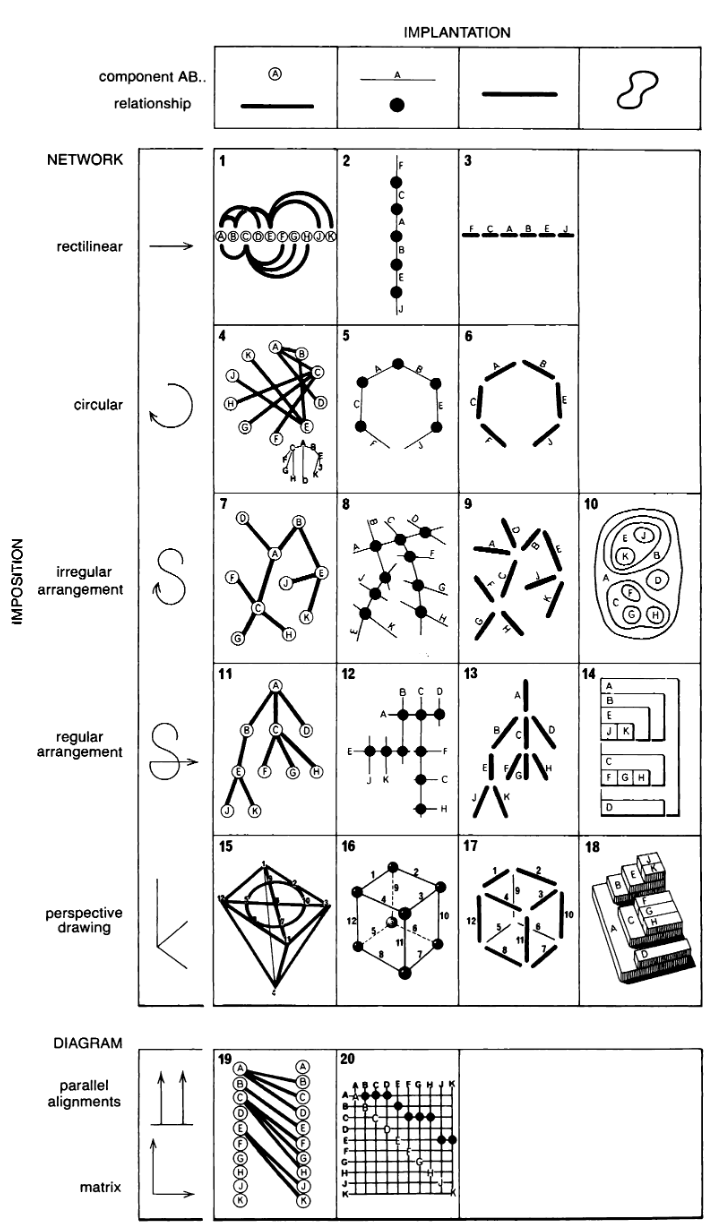
\includegraphics[width=0.78\textwidth]{static/figures/RelatedWork/BertinNetworks}
    \caption{Categorization of visual variables which can be used to represent network data, resulting in many different network representations. Image from \cite{bertin1967}.}
    \label{fig:bertin-network}
\end{figure}

In this foundational work, Bertin described and organized the different visual elements usable in graphical information displays, and linked them to data features and relations types.
An illustration of this work of categorization for network data is illustrated in \autoref{fig:bertin-network}.
Michael Friendly writes ``To some, this appeared to do for graphics what Mendeleev had done for the organization of the chemical elements'' \cite{friendlyBriefHistoryData2008}.
The development of computer science and the rise of hardware capabilities at the same time created a big need for data visualization.
The amount of data stored increased exponentially \cite{hilbertWorldTechnologicalCapacity2011} and descriptive statistics were not enough to understand the underlying structure of the amount and diversity of produced data.
Visualization, leveraging the human visual system, enabled to rapidly see the hidden structure of a dataset and detect interesting and unexpected patterns very often unseen with classical statistical methods.
One classical illustration of this is Anscombe's quartet\cite{anscombeGraphsStatisticalAnalysis1973} which consists of four datasets of 11 points in $\mathbb{R} ^{2}$ with the same statistical measures (mean, variance, correlation coefficient, etc.) but with very different structures, that are immediately revealed when plotting the data.
The four datasets are illustrated in \autoref{fig:anscombe-quartet}.

\begin{figure}
    \centering % avoid the use of \begin{center}...\end{center} and use \centering instead (more compact)
    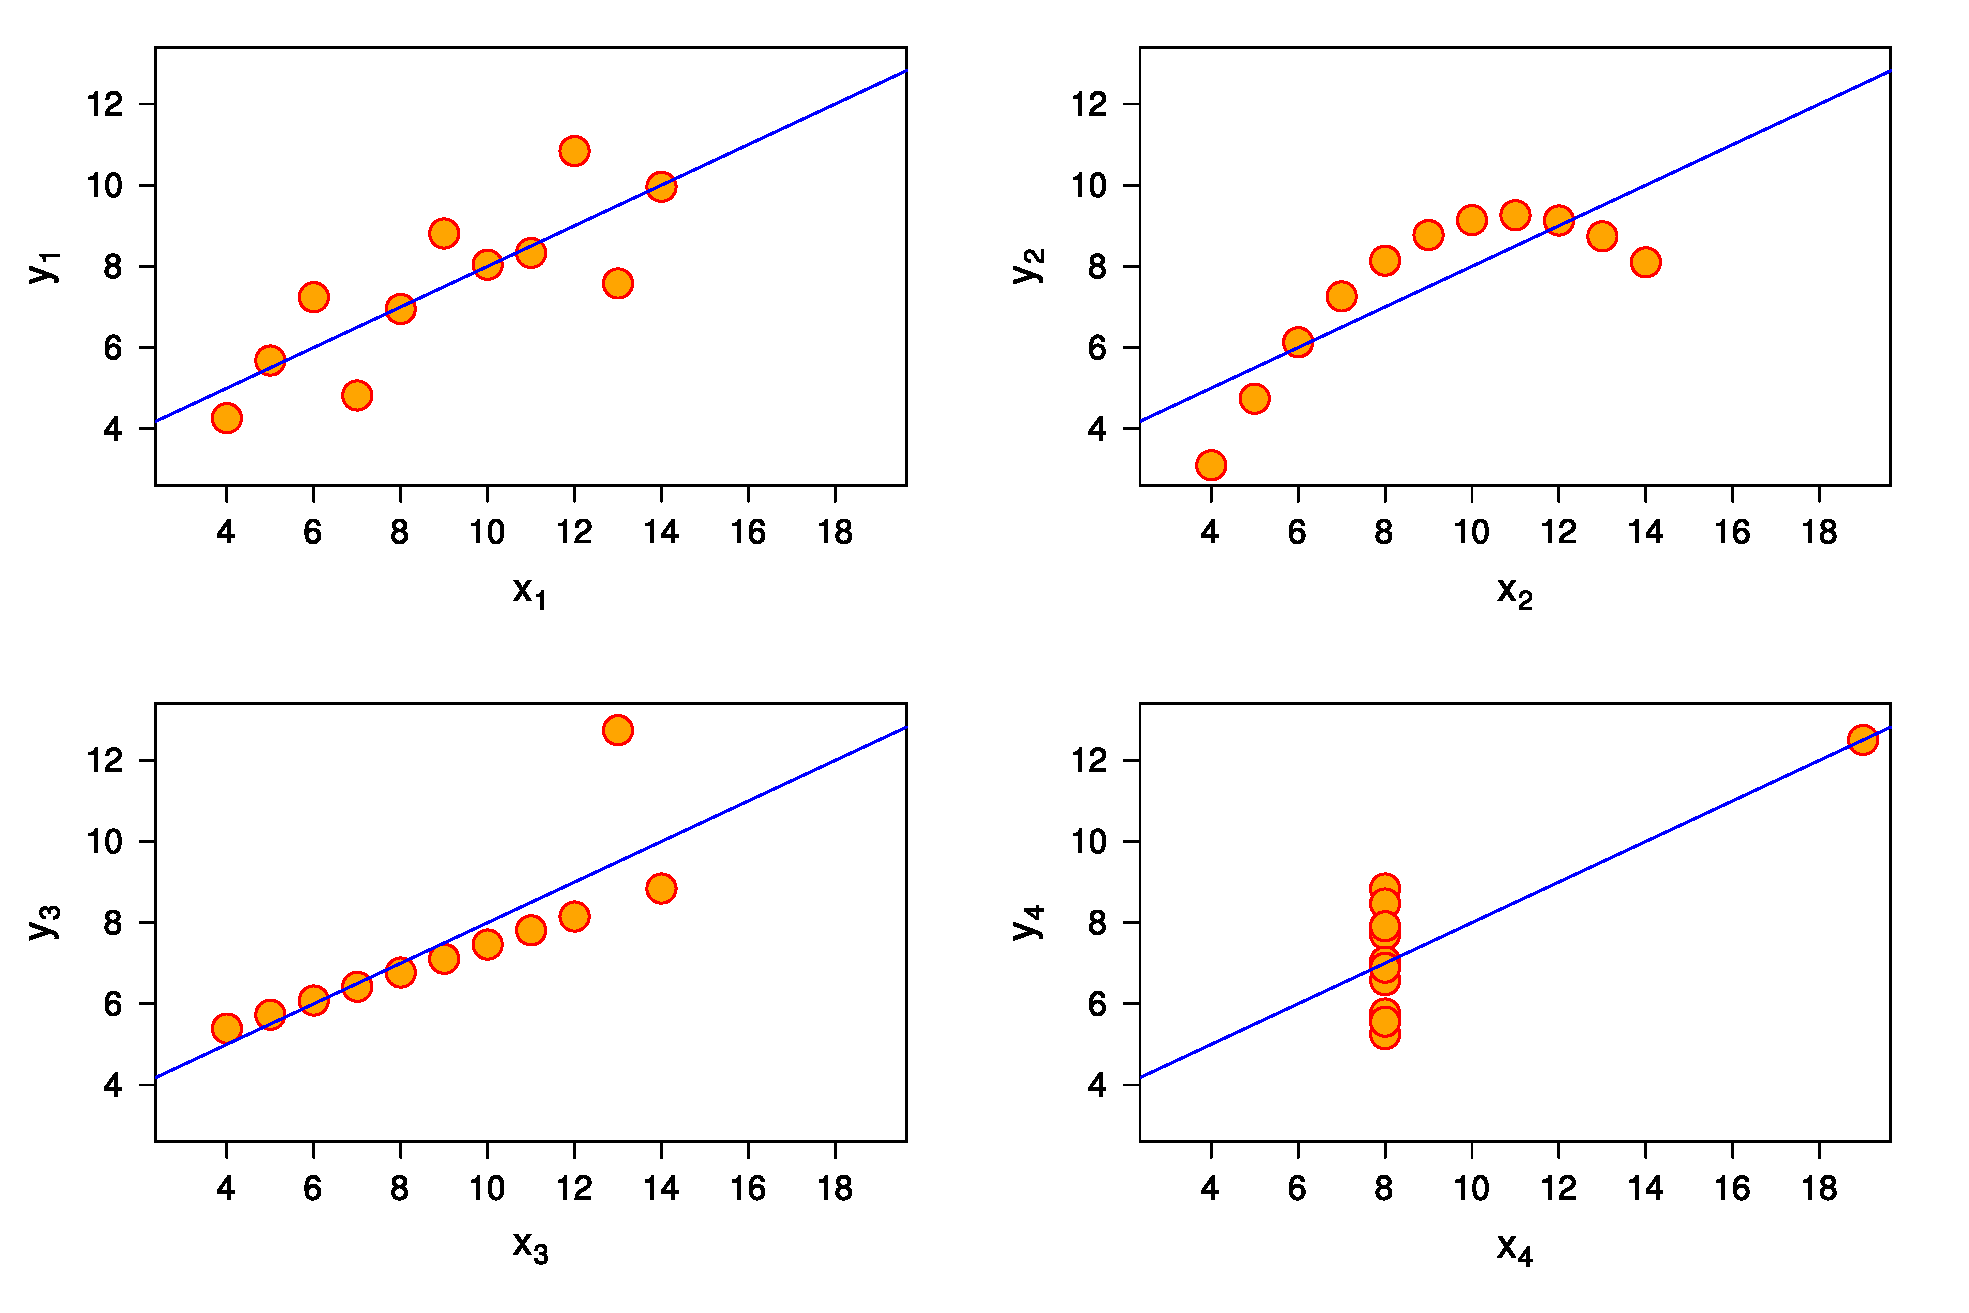
\includegraphics[width=0.8\textwidth]{static/figures/RelatedWork/Anscombe.pdf}
    \caption{Anscombe quartet. The four datasets have the same descriptive statistics (average, variance, correlation coefficient) but very different structures. Image from \cite{anscombeGraphsStatisticalAnalysis1973}.}
    \label{fig:anscombe-quartet}
\end{figure}

A large number of visualization techniques emerged to make sense of the diversity of data produced, such as multidimensional, temporal, spatial, or network data \cite{shneidermanEyesHaveIt1996}.
Instead of using taxonomies classifying graphics into categories such as histograms, pie charts, and stream graphs, some theorized how to describe graphics in a more systematic and structural way.
In 1993, Wilkinson extended Bertin's work and developed the Grammar of Graphics \cite{wilkinsonGrammarGraphics1993} as a way to describe the deep structure unifying every possible graphic, thus allowing to characterize and create graphics using common terms and rules.
In this framework, a graphic can be defined as a function of six components: data (a set of data points and attributes from a dataset), transformations (statistical operations which modify the original data, \eg mean and rank transformations), scales (\eg linear and log scales), coordinate systems (\eg cartesian and polar coordinate systems), elements (graphical marks such as rectangular or circular marks, and their aesthetics, \eg color, and size), and guides (additional information such as axes and legend).
Many well-known visualization toolkits are now based on this framework, such as vega\cite{satyanarayan2016vega} and ggplot\cite{wickham2007ggplot}, as it allows greater expressiveness and reusability for graphic creation.
Visualization allows to gain insight into the structure of a given dataset and has traditionally been used for confirmation and communication purposes, for example, to verify hypotheses on empirical sciences, and later on to communicate findings, first to scientific peers, and nowadays to broader audiences for example through the means of data journalism\cite{bradshawDataJournalism2017}.
%Since the 1960s, visualization is also used for exploration to generate new insight


%Subfields of Visualization emerged: \textbf{Scientific visualization} focus on visualizing continuous real data such as weather, spatial, and physics data, sometimes produced with simulations whereas \textbf{Information Visualization} is centered around the visualization of (multidimensional) discrete data points, often in an abstract way. \textbf{Visual Analytics} emerged later from Information Visualization by mixing data mining and more complex analysis process with traditional information visualization displays.
%Historical Social Network visualization is closely related to Information Visualization and Visual Analytics, and good visualization systems for HNR use concepts and methodologies from those two fields.


\subsection{Visual Analytics}

\va consists of the coupling of visualization and data mining techniques to better support users in their knowledge generation process through continuous interaction with the data and statistical models\cite{thomasVisualAnalyticsAgenda2006}.
It draws inspiration from exploratory visualization, interaction, and data mining.
The process of exploratory visualization to gain new insights on the general structure of the data and potentially generate new hypotheses has been characterized by Tukey in 1960 as \emph{Exploratory Data Analysis}\cite{tukeyExploratoryDataAnalysis1977}.
It consists in trying to characterize the structure of a dataset with the help of continuous visualization and statistical measurements of different dimensions of the data.
Visual exploration is enhanced by direct manipulation interfaces through interaction and usually follows the information-seeking mantra formalized by Schneiderman: ``Overview first, zoom and filter, then details-on-demand'' \cite{shneidermanEyesHaveIt1996}.
It allows users to first have a visual overview of the data and get an idea of its overall structure, to then change the point of focus to highlight interesting patterns with the help of filtering, querying, sorting, and zooming mechanisms.
%Exploration is enhanced by direct manipulation interfaces and interaction, which allows changing the point of focus in the data to highlight interesting patterns, with the help of filtering, querying, sorting, and zooming mechanisms.
As the average size of datasets keeps growing, exploratory tools are often needed to make sense of large datasets and generate pertinent hypotheses.

%Moreover, with the develpment of data mining and machine learning methods,
%Social scientists also often want to gain insight with the help of statistical and machine learning methods, that visualization only can not provide.
More recent visual exploration interfaces also incorporate automatic analytical tools along with graphical displays, letting users apply data mining algorithms directly in the exploratory loop.
This coupling of visualization and analytical methods such as data mining has been defined as Visual Analytics (VA) and is still a very active research field.
Keim and al.\ define it as ``a combination of automatic and visual analysis methods with a tight coupling through human interaction in order to gain knowledge from data'' \cite{keimVisualAnalyticsDefinition2008}.

\begin{figure}[!ht]
    \centering % avoid the use of \begin{center}...\end{center} and use \centering instead (more compact)
    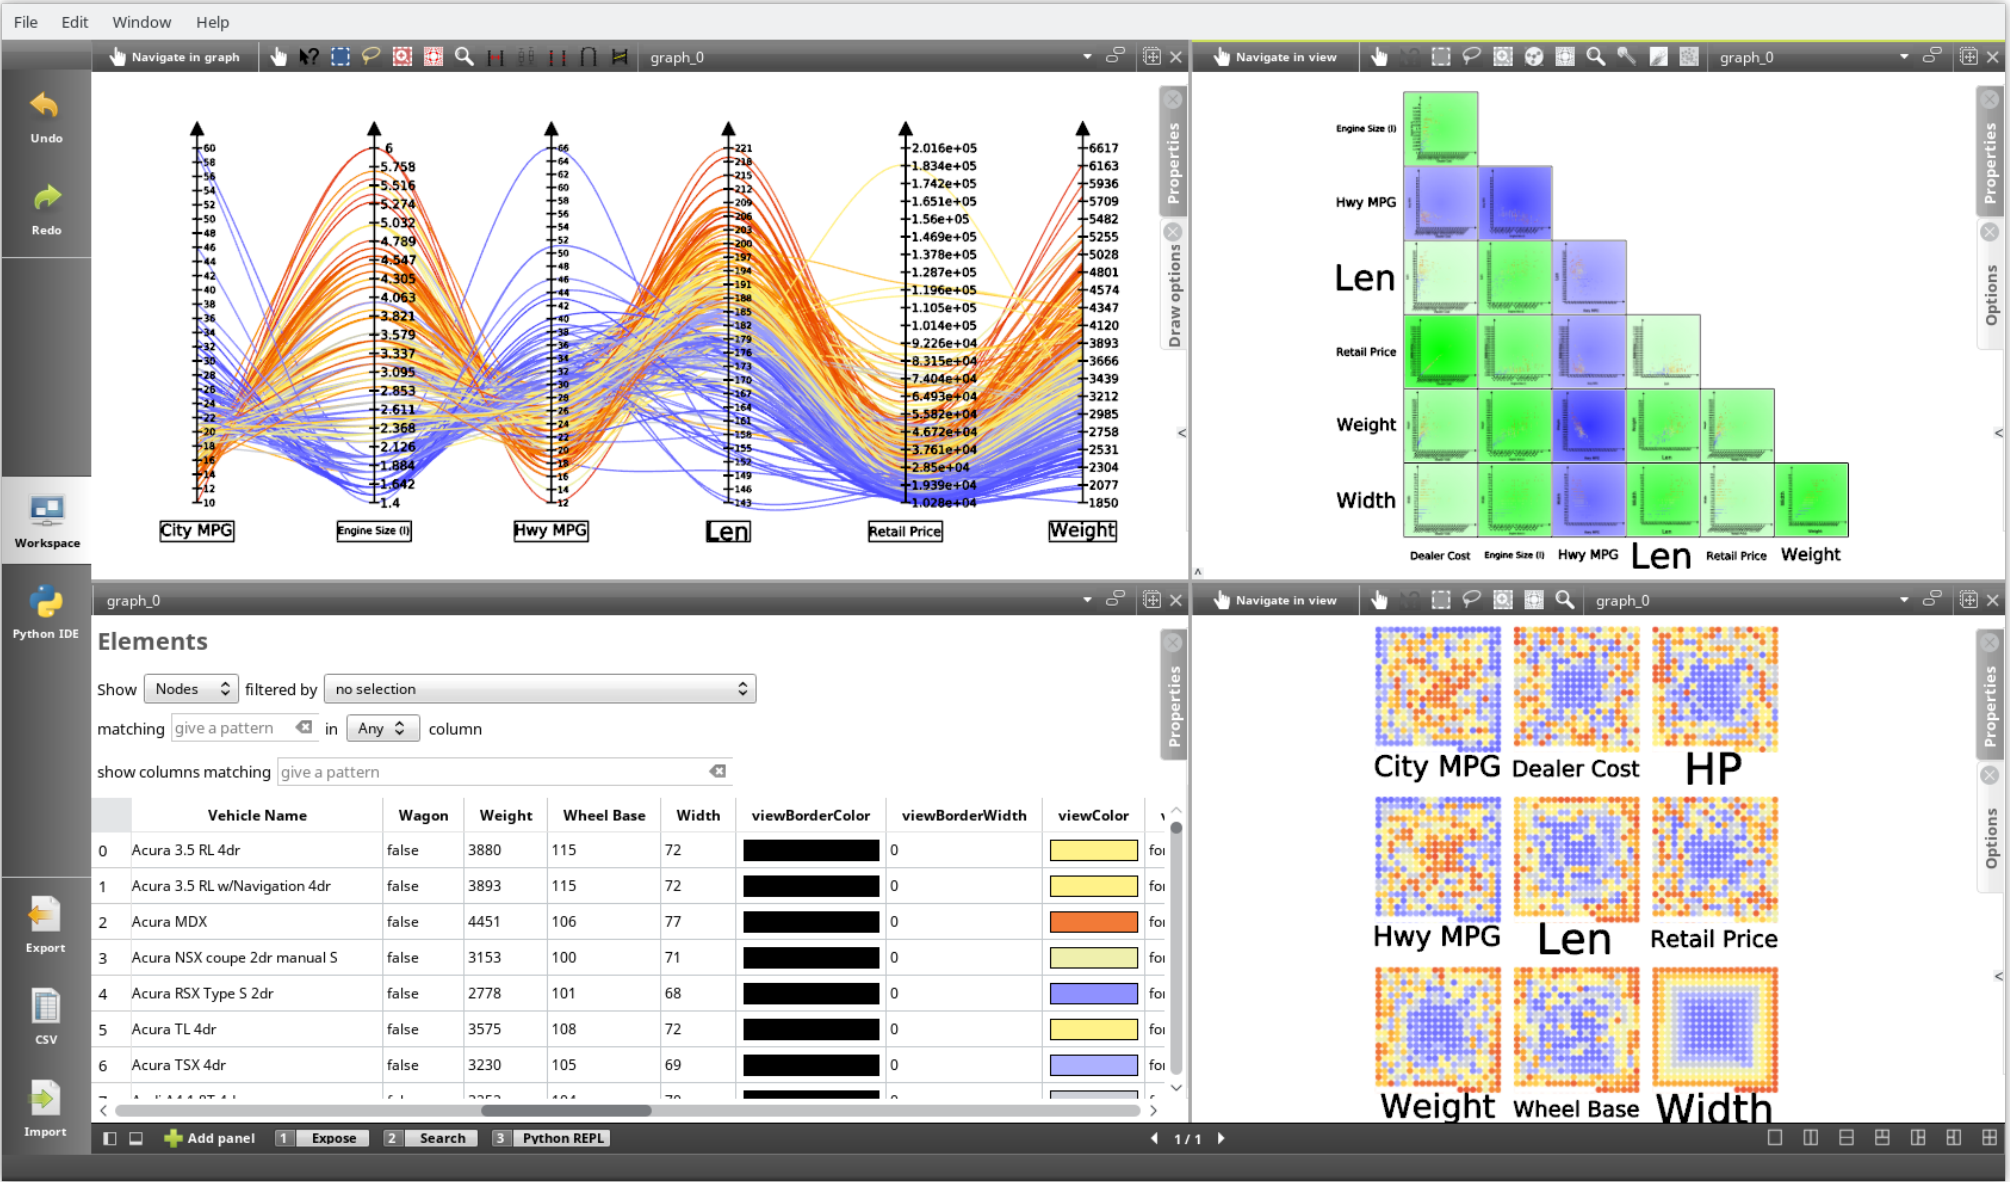
\includegraphics[width=1\textwidth]{static/figures/RelatedWork/TULIP}
    \caption{TULIP software is designed for application-independent network visual analytics\cite{auberTULIP2017}. The view shows a dataset among multiple interactive coordinated views. Users can also apply data mining algorithms on the data to extract interesting patterns.}
    \label{fig:RW-tulip}
\end{figure}

\va consists of the generation of knowledge using visualizations and statistical models of the data, that the user can explore using interaction.
Such systems have been developed in various empirical domains, such as biology, astronomy, engineering, and social sciences, to explore various data types: multidimensional, temporal, geolocated, or relational (\ie modeled into a network).
\autoref{fig:RW-tulip} shows the TULIP system, an example of a \va system developed for the analysis of network data.
We discuss the uses of \va specifically for \hsna in \autoref{subsec:social-network-visual-analytics}
%as it allow to rapidly gain insight on the structure of various potentially large dataset, while generating and refuting hypotheses.

%but are nonetheless not used by the majority of application scientists.
%Indeed, there are currently debates on the roles of EDA and VA in the scientific process, as exploratory findings do not have the same level of proof than statistical results coming from the hypothetico-deductive model.
%\eda and \va are nevertheless efficient tools to refute and generate hypothesis, especially with the ever-increasing amount of stored data.


%Social scientists now frequently use VA systems to make sense of their data by using visualization, interaction, and data mining algorithms in their analysis loop to find interesting patterns and verify and create hypotheses.
%The most used social network VA tools are Gephi \cite{Gephi}, Pajek \cite{mrvarAnalysisVisualizationLarge2016}, and NodeXl \cite{NodeXL}. \autoref{fig:gephi} presents the Gephi interface showing a clustered social network, where each node is part of a cluster, encoded by color.
%They all let users visualize their networks with a node-link diagram, and allow an interactive exploration of the data with operations like filtering.
%Users can also analyze their data using network measures computed directly in the interface, and apply data mining algorithms such as clustering which results are explorable visually.



\section{Quantitative Social History}\label{sec:social-history}


Social History is a branch of history that aims at studying socio-economic aspects of past societies, with a focus on groups instead of specific individuals only.
Charles Tilly writes that its goal is to ``(i) documenting large structural changes, (2) reconstructing the experiences of ordinary people in the course of those changes, and (3) connecting the two'' \cite{tilly1984retrieving}.
If the purpose of social history remained the same across time, methods and formalisms have evolved since its beginning in the 1930s.
Specifically, the rise of computer science led to the development of quantitative history methods in the 1960s---now often referred to as Digital Humanities---which brought new ways of grounding results in formalisms and quantitative models, instead of solely relying on qualitative inspection of historical documents \cite{haskinsUnderstandingQuantitativeHistory2011}.
We discuss in this section the evolution of social history from the context of its beginning to the use of more recent quantitative approaches.


%First social history studies emphasized the methodic extraction of historical documents from archives to ground results in the reality of the documents.
%Following the rise of computer science, historians started to use quantitative methods in the 1960s on data extracted from historical documents.


%If Sociology and Anthropology started to use network concepts and methods rapidly in the 1950s, it was not until the 1980s that historians started to use this type of methodology.
%Yet, historians started to use quantitative methods in the 1960s, with the rise of social history, by extracting information from historical textual documents and studying them with statistical methods.
%When seeing the potential of SNA concepts for historical purposes, historians started to extract the relational information contained in documents to study historical social phenomena using the power of networks and methods already developed in SNA.


\subsection{History, Social History, and Methodology}\label{subsec:history-and-social-history}

The concept of History is hard to define as its practice and codes highly evolved through time.
Prost writes ``History is what historians do. The discipline called history is not an eternal essence, a Platonic idea. It is a reality that is itself historical, i.e. situated in time and space, carried out by men who call themselves historians and are recognized as such, received as history by various publics \cite{prost2014}.''
Retrospectively, History of a given time can thus be characterized by the different historical work produced at that time.
Nevertheless, History can be characterized as the collection and study of historical documents to study and describe the past.
As Langlois and Seignobos write, ``The search for and the collection of documents is thus a part, logically the first and most important part, of the historian's craft'' \cite{langloisIntroductionAuxEtudes2014}.
History emerged as a field with its own rules, conventions, and journals in the 1880s from faculties of letters, to counterbalance previous history works which were judged as too ``literary'' \cite{noirielNaissanceMetierHistorien1990}.
At that time and until now, two facets characterize the field, which are sometimes overlapping: one is political whereas the other one is methodological.
%History can be seen through two facets: political and methodological.
The former aspect of history serves to create a shared story for the studied country and a sense of unity among its citizens.
Antoine Prost says that ``it's through history than France thinks itself''\cite{prost2014}.
%It is closely related to political power
The latter aspect of history constitutes a methodology to describe the past through methodical inspection of historical sources, with the aim of inferring dated facts about the past and trying to minimize possible bias.
%For this, historians rely on historical documents that they leverage to infer dated facts about the past (the temporal aspects of conclusions is always central to the historian work).
Historical documents are thus at the core of the work of historians and having to cite historical documents and previous peers' work for new claims is primordial to be considered rigorous History work.
However, methodological and epistemological facets (how historians should read and analyze their sources, how to cite them, what to report/not report, and what is the status of proof) of History have not been studied and discussed for a long time, until the end of the 1980s.
%However, even if those two aspects are well characterized (temporal aspect of the work and its relationships to sources), methodological and epistemological facets (how historians should read and analyze their sources, how to cite them, what to report/not report etc.) of History have not been studied and discussed for a long time, until the end of the 1980s.
Some historians were interested in historiography \cite{carbonellHistoriographie1981}, but none were going to philosophical and epistemological debates on the History discipline.
For Lucien Fèbvre, philosophizing was even constituting a ``capital crime'' \cite{febvreVERSAUTREHISTOIRE1949, prost2014}.
%Les historiens font ordinairement de l’histoire sans méditer sur les limites et les conditions de l’histoire  ; sans doute, ils ont raison ; il vaut mieux que chacun fasse son métier ; d’une façon générale, il vaut mieux qu’un historien commence par faire de l’histoire sans en chercher aussi long : autrement, il n’y aurait jamais rien de fait

%\alexis{maybe talk about the positivists and methodists}
Retrospectively, we can still observe shifts in the objects of study of historians through time, and their relation to sources.
History was at first mainly event-centered and was focusing on characterizing central figures of the past like rulers and artists or shedding light on central events like wars or political crises.
This narrative approach to history has been criticized for its open interpretation of historical documents, which can introduce bias from the authors \cite{bourdieuRapportsEntreSociologie1995}.
%Social History emerged as a sub discipline of history with a focus on the social ascpect of history, trying to link political events (such as a revolution) to
In the 1930s, March Bloch and Lucien Fèbvre detached from traditional history by creating the ``Annales school'' (\'Ecole des Annales) which aimed at placing the human as a component of a broader sociological, political, and economic system with influences on each other \cite{burkeHistorySocialTheory2005}.
They strongly advised exhaustively searching from archives, to ground historical results in documents, texts, and numbers.
This new way of studying past events and societies became successful in a profession in crisis, by bringing a new lens of study on various societal subjects more grounded in sources and with better intelligibility.
This school of thought can be seen as one of the biggest milestones for Social History, which focuses on the socio-economical aspects of societies and their changes through time, rather than an event-centric view of History.
For example, in his thesis, Ernest Labrousse---a well-known figure in Social History---tries to describe and explain the economic crisis of France at the end of the ``Ancien Régime''\footnote{The ``Ancien Régime'' is a historical period of France which starts from the beginning of the reign of the Bourbon house at 1589 until the Revolution in 1789.} through the evolution of the economic power of different social groups such as farmers, workers, property owners etc\. instead of solely describing memorable facts about the period \cite{labrousse1990crise}.
Social History continued to evolve since the 1930s, introducing new methods and concepts, but always with the goal to describe periods and historical facts through a sociological lens and with a strong focus on sources and traceability.


\subsection{Quantitative History}\label{subsec:quantitative-history}

%Historians try to understand an epoch using textual sources from the past, and trying to extract useful information from them.
%Social history, which is a branch of history, focus on understanding how societies were organised and how people were living together at a particular time and place. Charles Tilly argued that the task of social history lays in "(i) documenting large structural changes, (2) reconstructing the experiences of ordinary people in the course of those changes, and (3) connecting the two". For the latter, historians can leverage personal written sources---such as letters, journals, books, and newspapers---to have the internal point of view of persons living in this society and descriptions of lives of precise individuals.
%For the former, historians usually need to study more structured documents which contain information which can be extracted in a predefined and exhaustive way.
%These documents can for example be census, migration acts or marriage acts. By studying theses documents and by systematically extracting the information of these documents, historians can make global and quantitative conclusions on certain social and behavioural aspects of societies of interest.
%For example .. [EXAMPLE CHANGEMENT METIERS XXth century]

%Traditionally, historians try to tell a story about protagonists and socio-economic facts in a given society by reading, understanding, and linking together historical sources.
%This narrative approach to history has been criticized for its lack of traceability and the open interpretation of historical documents, which can introduce bias from the authors.
%To solve this problem, the ``Annales school'' (Ecole des Annales) proposed to characterize past social phenomena through the exhaustive and systematic analysis of historical documents~\cite{prost2014}.

With the development of statistical methods and Computer Science, quantitative approaches to History emerged in the 1960s with the goal of analyzing numeric data directly extracted from historical documents.
Economists led this first wave of quantification by studying past events using economical concepts and data.
This approach called ``new economic history'' or ``cliometrics'' was popularized by Fogel's study on the economic impact of the development of railroads in America\cite{fogelRailroadsAmericanEconomic1964} and Fogel and Engerman's controversial work on the economy of slavery\cite{fogel1974time}.
In the latter study, they extracted numbers of a sample of 5000 bills of slave sales from New Orleans to support the controversial claims that slavery was economically viable and that slaves had a decent material life, which brought up heated debate among the scientific community and the broad audience\cite{whaplesWhereThereConsensus1995}.
These kinds of approaches rapidly started to be used in other related domains such as demography, social history, and political history, sometimes rebranded as ``new social history'' and ``new political history''\cite{lemercierBackSourcesPracticing2021}
As extracting the data from raw documents and uploading it to computers---which were shared among whole departments---was very time-consuming at that time, ``new history'' projects often relied on a high division of labor among researchers, assistants, and students who operated with punch card operators\cite{landesHistorySocialScience1971}.
Many saw the future of social sciences in computer programming, as Le Roy-Ladurie who wrote in 1968 ``The historian of tomorrow will be a programmer, or he will not exist''\cite{lemercierQuantitativeMethodsHumanities2019}.

However, quantitative methods started to be criticized in the 1980s with a wave of disillusionment, for several reasons.
Stone was the first to raise his voice in 1979, after participating himself in several of those ambitious projects: ``It is just those projects that have been the most lavishly funded, the most ambitious in the assembly of vast quantities of data by armies of paid researchers, the most scientifically processed by the very latest in computer technology, the most mathematically sophisticated in presentation, which have so far turned out to be the most disappointing''\cite{stoneRevivalNarrativeReflections1979}.
First, many researchers of this first wave dispensed themselves with source criticism, leading to simplification, anachronisms---such as using modern analytical categories and indices like the GDP---and taking the numeric data from historical documents as objective.
These problems could be in part explained by the fact that the work process was highly divided, meaning that the people analyzing the data did not necessarily inspect and read the original historical documents in depth.
Secondly, the popularity of these methods made practitioners forget about the many biases inherent to statistics, such as the sampling bias, or the fact that historical data is essentially incomplete data.
This resulted in the computation of long data series and aggregates which were sometimes nonsensical given the gaps in the sources\cite{lemercierQuantitativeMethodsHumanities2019}.
Finally, many historians raised their voices against the study of long-term trends instead of focusing on specific events and individuals.
They challenged aggregation procedures and their assumptions, trying to go back to a more complex history by pointing out that phenomena have to be studied and understood through several scales\cite{trivellatoThereFutureItalian2011}.
Indeed, computing correlations and aggregates at a national level greatly simplify complex phenomena and misses specific group and individual related behaviors.
Still, if their adoption remains slow and sometimes criticized among historians, quantitative methods provide tools to store, explore, and analyze historical documents systematically if used appropriately (i.e.\ not trying to bias the analysis, and not losing the trace of the original sources), especially that those methods highly evolved since the 1960s.



%Using such methods, historians were able to make conclusions based on statistical results on topics such as demography \cite{henryRegistresParoissiauxHistoire1956} or job distribution.
%For example, Gribaudi and Blum illustrated a shift in the most widespread professions in France during the 19th century using the data extracted from 50000 marriage acts \cite{gribaudi1990} and using statistical methods.


% TODO: put somewhere?
%Guildi and Aritage went as far as criticizing the decrease of interest of historians working in archives \cite{guldiHistoryManifesto2014}.
%Approaches using digital methods and tools are nonetheless more and more popular, sometimes more recently referred to under the umbrella term Digital Humanities (DH).



\subsection{Digital Humanities}\label{subsec:DH}

Digital Humanities is sometimes described as the second wave of computational social sciences \cite{lemercierQuantitativeMethodsHumanities2019}.
The term has gained popularity since the 2010s and refers to ``\textit{research and teaching taking place at the intersection of digital technologies and humanities. Digital Humanities aims to produce and use applications and models that make possible new kinds of teaching and research, both in the humanities and
in computer science (and its allied technologies). Digital Humanities also studies the impact of these techniques on cultural heritage, memory institutions, libraries, archives and digital culture.}'' \cite{terras2011quantifying}.
If the first wave of computational social sciences focused a lot on statistical methods such as regression models, correlation testing, and descriptive measures (mean, median, and variance) to make conclusions, digital humanities focuses more on the use of digital tools for exploration, teaching, and communication of humanities datasets and concepts, leveraging design, infographics, and interactive systems \cite{burdickDigitalHumanities2016}.
In the context of historical research, the term Digital History has been coined as ``\textit{an approach to examining and representing the past that works with the new communication technologies of the computer, the Internet network, and software systems. On one level, digital history is an open arena of scholarly production and communication, encompassing the development of new course materials and scholarly data collections. On another, it is a methodological approach framed by the hypertextual power of these technologies to make, define, query, and annotate associations in the human record of the past. To do digital history, then, is to create a framework, an ontology, through the technology for people to experience, read, and follow an argument about a historical problem.}'' \cite{InterchangePromiseDigital2008}
%Digital History therefore focus a lot on the curation and exploration of historical archives in the purpose of characterizing and communicate of historical concepts.
Research that label itself as Digital History pivots around the curation and digitization of historical archives, the identification of historical concepts through computational and exploration methods, but also their communication to the general audience through digital technologies.
\begin{figure}[!ht]
    \centering % avoid the use of \begin{center}...\end{center} and use \centering instead (more compact)
    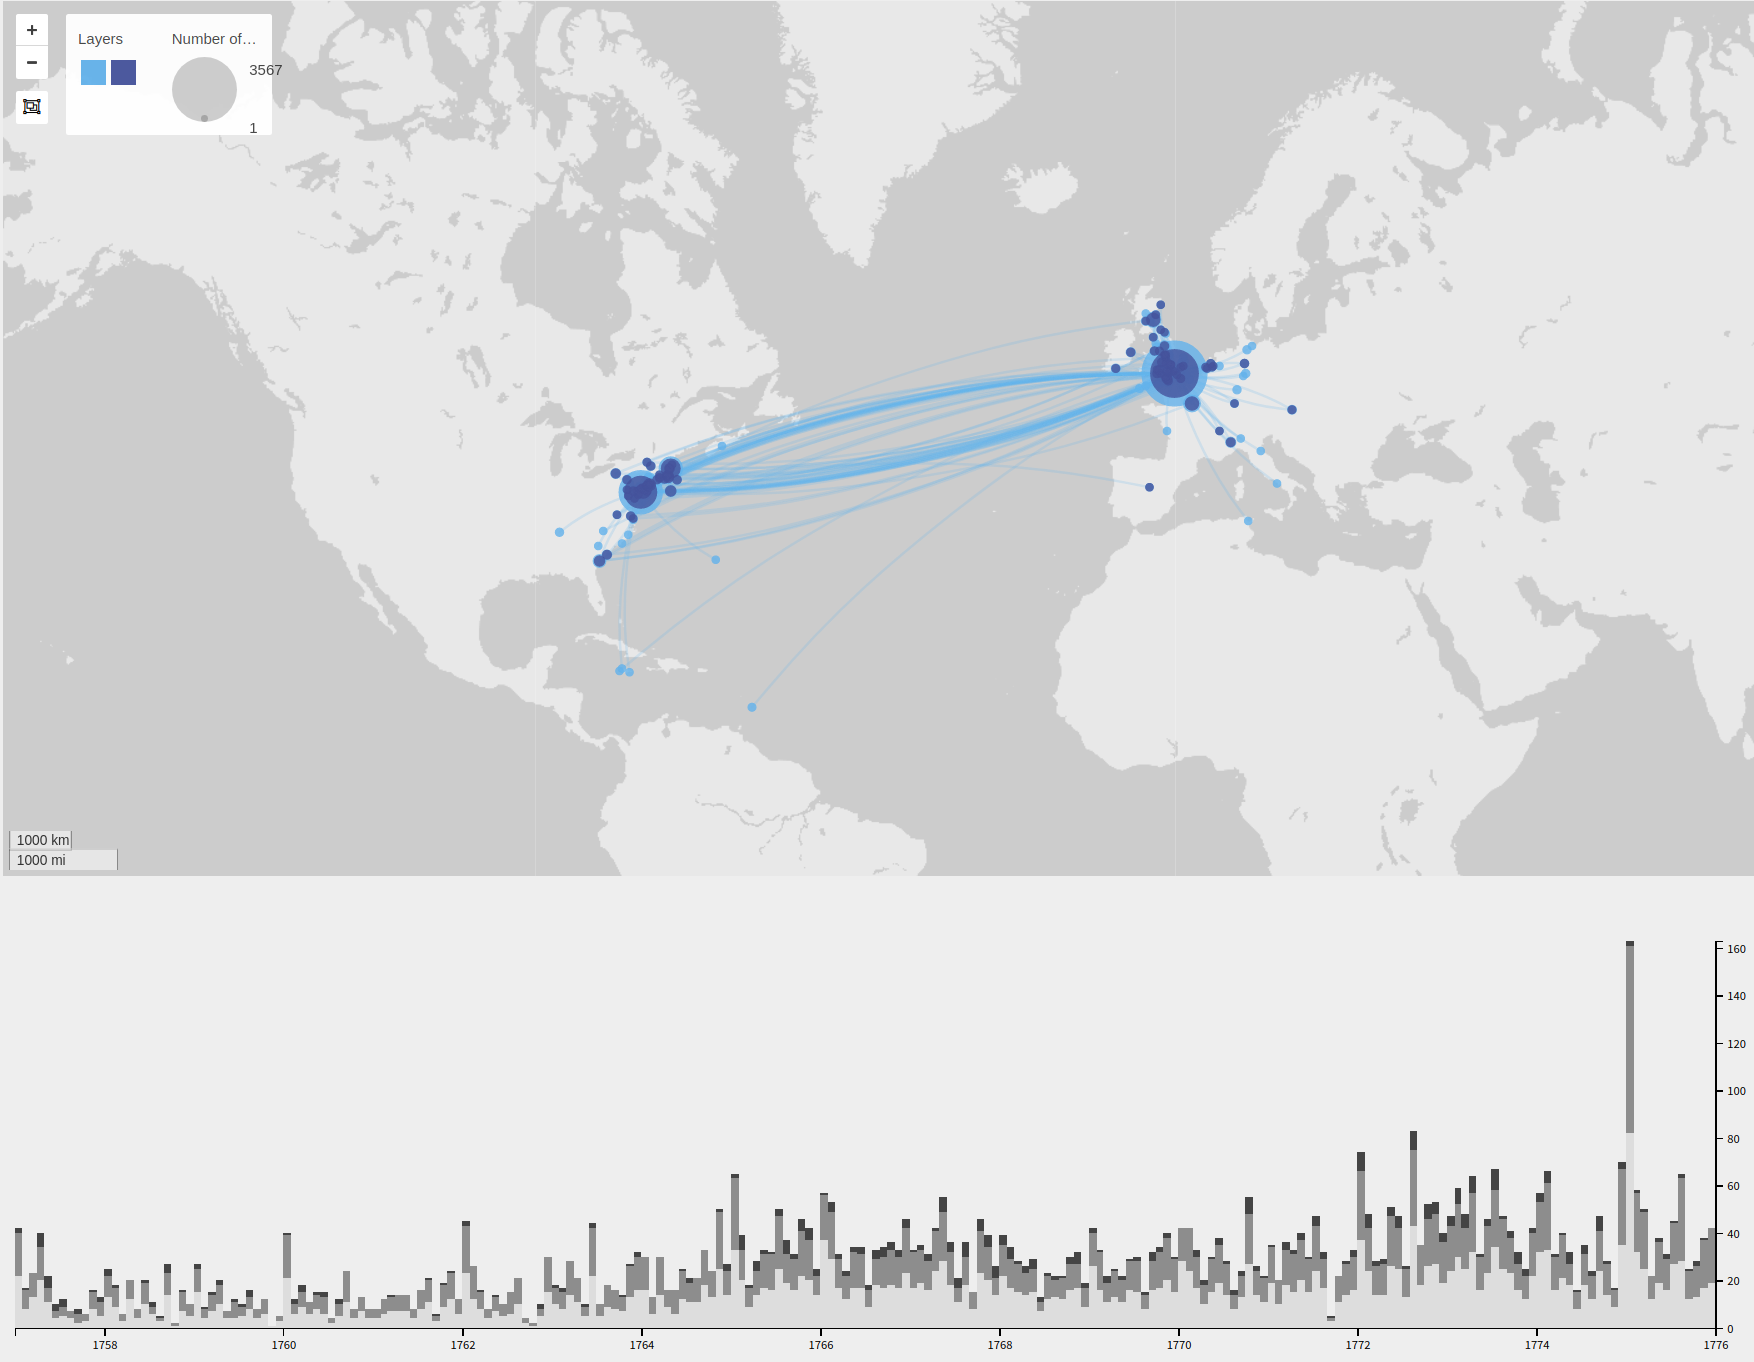
\includegraphics[width=1\textwidth]{static/figures/RelatedWork/RepublicOfLetter_BenjFranklin}
    \caption{Correspondence letters of Benjamin Franklin and his close relationships, visualized with a map and a histogram, accessible online on the republic of letter website\cite{edelsteinHistoricalResearchDigital2017}.}
    \label{fig:republic-letters}
\end{figure}
Many Digital History projects are thus multidisciplinary by essence and involve several teams of researchers, such as the Republic of Letters project which consisted of digitizing, storing, and exploring letters of scholars across the world, in a common hub and using shared visualization tools \cite{edelsteinHistoricalResearchDigital2017}.
It resulted in the elaboration of curated datasets and visualizations concerning the correspondence of various scholars such as Voltaire, Benjamin Franklin (see \autoref{fig:republic-letters}), and John Locke, accessible in the same place by researchers and the general audience.
With modern technologies and infrastructures, it also becomes possible to study large historical databases---often labeled under the term ``big data''---as with the Venice Time Machine project~\cite{kaplanVeniceTimeMachine2015} which aims at digitizing and analyzing thousands of documents from the archives of Venice to understand the political, geographical, and sociological dynamics of the cities across generations and centuries.
Yet, some historians raised concern about this type of project, fearing that it could rapidly bring the same type of issues that we saw during the first wave of quantification, especially for big projects involving many actors and highly ambitious goals\cite{lemercierQuantitativeMethodsHumanities2019}.

Many projects which claim themselves as Digital History also leverage new methods compared to the 1960s and 1970s, such as the use of network methods and concepts \cite{ahnertNetworkTurnChanging2020}.
Examples are the Viral Texts \cite{cordell2017viral} and Living with Machines \cite{ardanuyLivingMachinesStudy2020} projects which respectively study nineteenth-century newspapers and the industrial revolution by translating their sources into analyzable networks.
We discuss more in detail the related work of network analysis for historical research in \autoref{sec:hsna}.


\section{Historical Social Network Analysis}\label{sec:hsna}

Historians started to use network analysis to study relational structures and phenomena of past societies in the 1980s, using similar methods developed by sociologists under the label of \sna.
\sna is defined as an ``\textit{approach grounded in the intuitive notion that the patterning of social ties in which actors are embedded has important consequences for those actors. Network analysts, then, seek to uncover various kinds of patterns. And they try to determine the conditions under which those patterns arise and to discover their consequences}'' \cite{freemanDevelopmentSocialNetwork2004}.
the use of networks emerged in response to traditional sociology methods using pre-defined taxonomies and social categories to understand and explain sociological behaviors and phenomena, which could introduce bias.
By modeling real observed social relationships and interactions with networks and by using mathematical and statistical methods to study those, sociologists have been able to explain sociological phenomena and describe sociological interactions through their direct observation modeled as networks.
%SNA is now a well-praised methodology in sociology, which has also been extended to History to study relational aspects of societies and institutions of the past.
\sna is now a well-praised methodology in sociology and has been extended to historical research to study relational concepts such as kinship, friendships, and institutions of the past.
Social historians leverage their documents to extract relationships between entities---often persons---that they model into networks.
Leveraging network measures and visualization, they can make conclusions through structural observations of such networks.


\subsection{Sociometry to SNA}

One of Sociology's main goals is to study social relationships between individuals and find recurrent patterns and structures allowing us to generalize on how social relations operate, and what are the social specificity of specific groups and individuals\cite{scottSocialNetworkAnalysis1988}.
Traditional methods try to answer those questions using classical social classifications such as age, social status, profession, and gender, typically collected from surveys and interviews.
Criticism pointed out that this type of division is often partially biased and comes from predefined categories which are not always grounded in reality\cite{freemanDevelopmentSocialNetwork2004} and that using random sampling of individuals with such methods remove them from their context.
The sociologist Allen Barton wrote in this regard ``For the last thirty years, empirical social research has been dominated by the sample survey. But as usually practiced, using random sampling of individuals, the survey is a sociological meatgrinder, tearing the individual from his social context and guaranteeing that nobody in the study interacts with anyone else in it''\cite{bartonSurveyResearchMacroMethodology1968}.
Sociometry is considered one of the bases of \sna and had the goal of redefining social categories through the lens of real social interactions and ties between persons, which sociologists wanted to observe in real conditions.
It is in the 1930s that Moreno started to develop this new method by trying to depict real social interactions as a way to understand how groups and organizations were socially structured\cite{morenoFoundationsSociometryIntroduction1941}.
He developed sociograms to visually show friendships between people with the help of circles representing persons and lines modeling friendships.
\begin{figure}[!ht]
    \centering % avoid the use of \begin{center}...\end{center} and use \centering instead (more compact)
    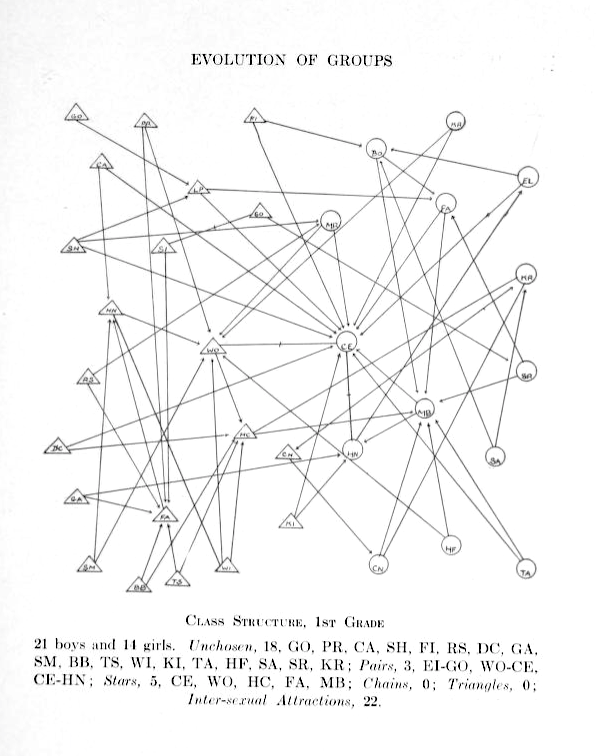
\includegraphics[width=0.45\textwidth]{static/figures/RelatedWork/Moreno-1}
%    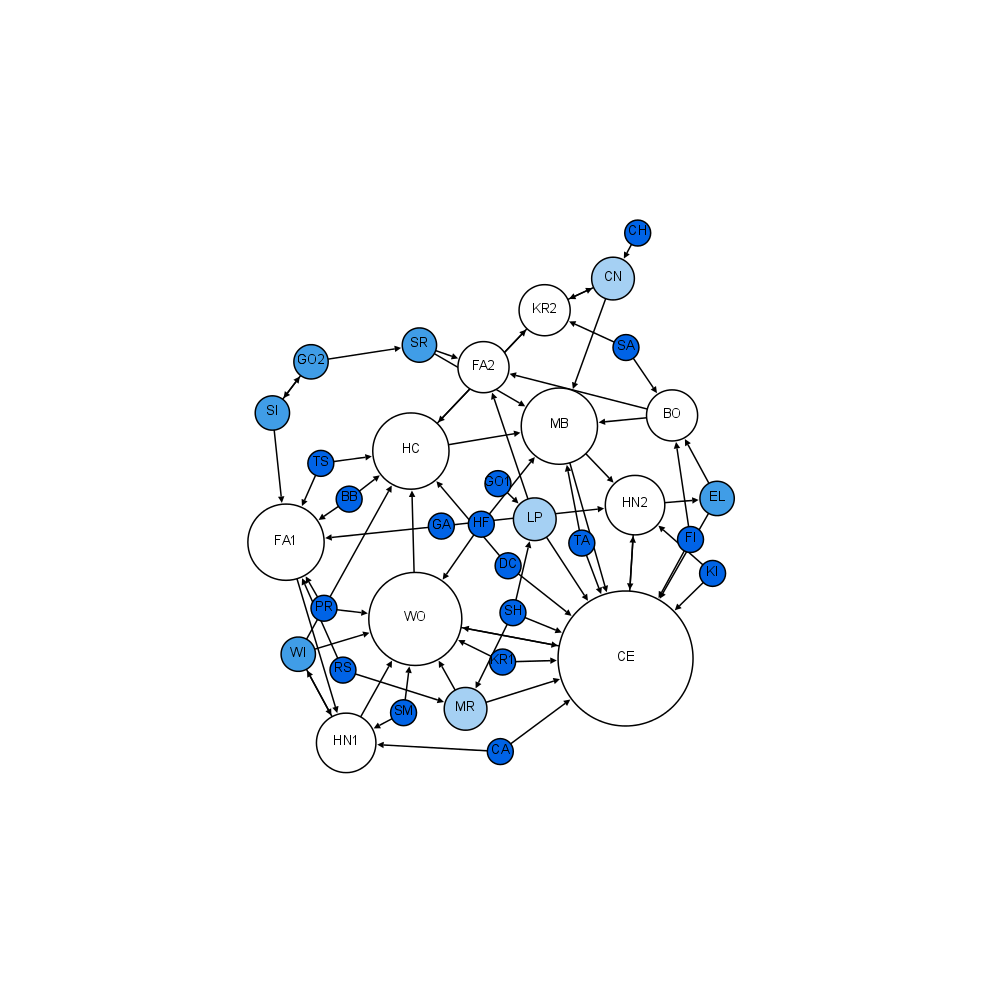
\includegraphics[width=0.55\textwidth]{static/figures/RelatedWork/Moreno-1_GrandJean}
    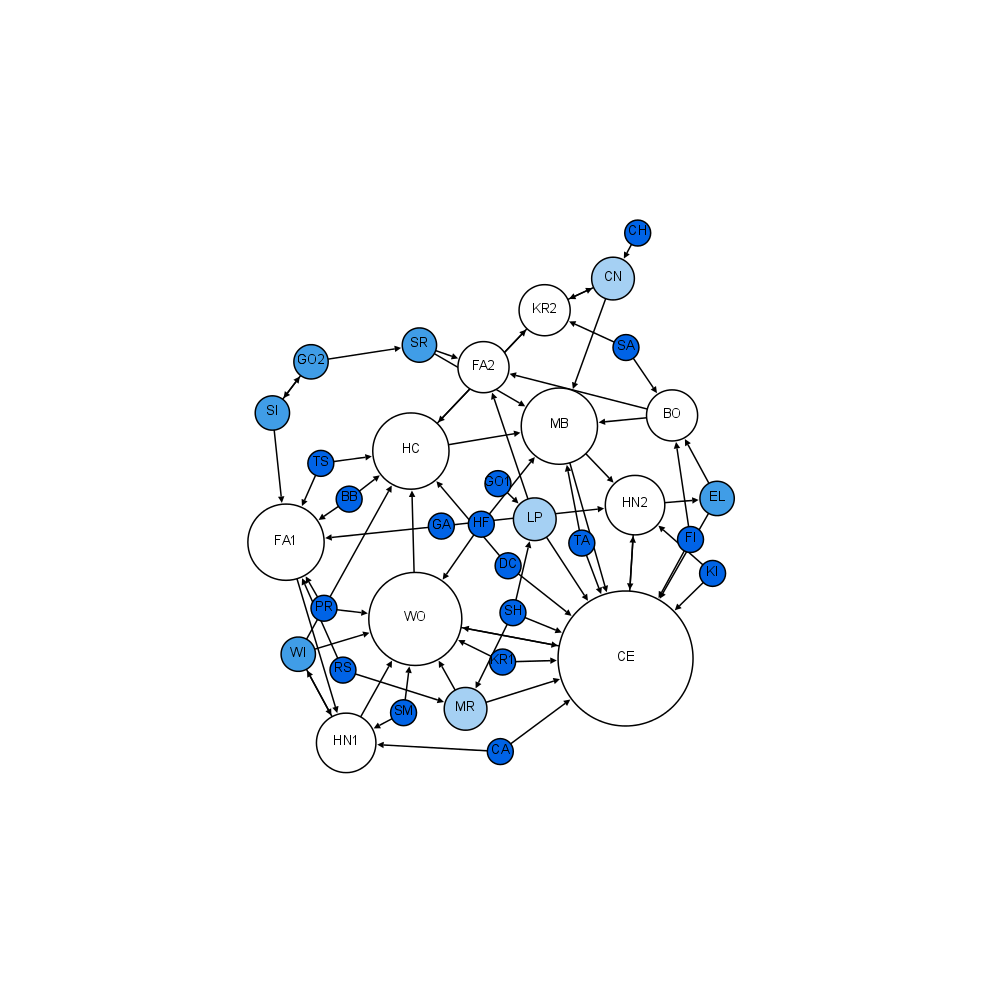
\includegraphics[width=0.50\textwidth,trim={4cm 4cm 4cm 4cm},clip]{static/figures/RelatedWork/Moreno-1_GrandJean}
    \caption{Moreno's original sociogram of a class of first grades from \cite{morenoWhoShallSurvive1934} (left). The diagram shows 21 boys (triangles) and 14 girls (circles). The same sociogram using modern practices generated from Gephi from \cite{grandjeanSocialNetworkAnalysis2015} (right). The color encodes the number of incoming connections.}
    \label{fig:moreno-sociogram}
\end{figure}
\autoref{fig:moreno-sociogram} shows one of Moreno's original sociograms to depict friendships in a class of first grades (left).
%This way, he could rapidly see the main actors and hubs of interaction inside the social network represented visually.
Sociometry tremendously helped disseminate the metaphor of networks to model and understand social structures and phenomena.
It was during the 1960s that sociologists and anthropologists took these concepts further and formalized \sna using graphs\footnote{Graphs and networks refer to the same thing but are often used in different contexts. The term graph is preferred in a mathematical and abstract setting, while the term network is mostly used when modeling real-world phenomena. We talk about nodes and links for networks and vertices and edges for graphs.} and mathematical methods\cite{cConceptUseSocial1969, freemanDevelopmentSocialNetwork2004}, following the emergence of Graph Theory studies in the 1950s by Mathematicians such as Erd\H{o}s \cite{erdos2011}.
%It did not take long until sociologists used these concepts to model social ties and relationships into graphs.
Sociologists already had structural theories of social phenomena, and they rapidly saw the potential of graphs to model social relationships between actors of interest.
Typically, a graph is noted

\begin{equation}
    G = (V, E)\label{eq:graph}
\end{equation}

with $V$ a set of vertices representing the actors of interest---typically persons---and $E \subseteq V^2$ a set of edges modeling social relationships.
This simple model which does not take into account the diversity and extent of social relationships still allows the characterization of the sociological structure of groups and institutions---which is the primary focus of \sna\cite{scottSocialNetworkAnalysis1988, freemanDevelopmentSocialNetwork2004}.
More complex network models have been proposed with time to better take into account concrete properties of social relationships.
%such as the importance of actors or relations with weighted networks, multiple relationships with multiplex networks, dynamics of relations with dynamic networks.
I discuss those more in depth in \autoref{subsec:network-modeling}.

%representing the persons as nodes and relationships as links.
%Sociologists already had structural theories of social phenomena, and they rapidly saw the potential of graphs to model social relationships between actors, representing the persons as nodes and relationships as links.

Graph theory brought a panoply of concepts and methods to characterize the structure of  networks, that sociologists such as Coleman started to codify to use in a sociology setting\cite{colemanIntroductionMathematicalSociology1964}.
The use of network measures let sociologists explain social phenomena through the formal description of real observations of relationships modeled as networks.


\subsection{Methods and Measures}\label{subsec:methods-and-measures}

%After SNA started to be formalized, lots of sociological studies used those concepts.
%Many sociological studies used SNA concepts after it has been formalized.
%However, there were not yet strong protocols and methods to follow, and networks are an abstraction that can model different things in different ways.
%When looking retrospectively, we can see that two schools of thought emerged with different objectives and methods: the structuralists and the school of Manchester \cite{eveDeuxTraditionsAnalyse2002, maurizio2000, freemanDevelopmentSocialNetwork2004}.

Many measures and algorithms have been proposed in the network science and \sna literature to characterize the structure of simple networks as defined in \autoref{eq:graph} and relate it to social behaviors and phenomena\cite{scottSocialNetworkAnalysis1988, tabassumSocialNetworkAnalysis2018}.
Network measures are either global or local, which allows one to either make high-level conclusions on the general structure of social relationships or individual behaviors.
Widely used global measures include for example the density and the diameter, which give insight into the sparsity of the network and how distant on average are two random pairs of nodes.
Conversely, local measures give information on the structural position of a node compared to the rest of the network.
Centrality---probably the most used local measure---allows to formally compute a measure of how important or central are individuals in the network\cite{newmanNetworks2018}.
As defining what an important node is ambiguous, several types of centrality have been proposed such as the degree, betweenness, and closeness centrality, which respectively measure the number of connections, how nodes connect to different groups, and how close are the nodes compared to the rest of the network.

More generally, sociologists aim at identifying recurring patterns of sociability between actors and linking them to other behaviors, measures, or qualitative knowledge.
These patterns can for example be small unconnected components, cliques, or bow-tie structures.
Groups of nodes similarly located (central or distant) and having similar shapes are sometimes referred to as structurally equivalent\cite{lemercier12FormalNetwork2015}.
Instead of observing complex shapes, network scientists have also been interested in studying relationships at the lowest possible scale, \ie observing relations between sets of 2 and 3 nodes at one, also called dyads and triads\cite{wassermanSocialNetworkAnalysis1994}.
%The concepts of dyads and triads counting, which are basic structural patterns of 2 and 3 nodes, give insights into low-level relationships between people.
This reflects Simmel's formal sociology, where he already referred to dyads and triads as the primal form of sociability\cite{Simmel2013}.
More recently, graphlet analysis extended this concept to every pattern of N-entities\cite{pržuljBiologicalNetworkComparison2007}.

Graphlets are defined as small connected \emph{induced}, \emph{non-isomorphic} subgraphs composing any network\cite{miloNetworkMotifsSimple2002}.
In an \emph{induced} subgraph, two vertices linked in the original graph remain linked in the subgraph.
For instance, if the original graph is a triangle \TRIANGLE\ we can only induce the simple edge \EDGE\ or triangle \TRIANGLE\ subgraph (graphlet).
The path of length 2 \PATH\ has all vertices of the original graph but misses an edge and is, therefore, not a possible graphlet.


%Graphlet analysis aims at enumerating every small structure of $N$ nodes composing a network, to understand the local structures shaping the network.

\begin{figure}
    \centering % avoid the use of \begin{center}...\end{center} and use \centering instead (more compact)
    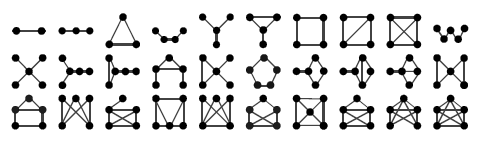
\includegraphics[width=1\textwidth]{static/figures/RelatedWork/all_graphlets_undir5}
    \caption{All possible graphlets of size 2 to 5 for undirected graphs}
    \label{fig:undir5-graphlets}
\end{figure}

\autoref{fig:undir5-graphlets} shows all graphlets of size 2 to 5, for undirected networks.
Graphlets counting shows that graphlets are not found in a uniform distribution in social networks\cite{charbeyStarsHolesPaths2019}, thus revealing that social networks do not have the same structure that random networks.
Precisely, entities in real-world networks tend to agglomerate into groups (also called clusters) where entities in the same groups interact more between them than with entities from other groups\cite{girvanCommunityStructureSocial2002}.
From a sociological perspective, it means that people tend to interact and socialize in groups and interact more rarely with other people from outside groups.
These groups are often referred to as \emph{communities}, and many algorithms have been proposed to find these automatically\cite{fortunatoCommunityDetectionGraphs2010}.

However, network concepts, measures, and algorithms have not been used only to study groups, organizations, and societies, but also to focus on separate specific individuals.
Indeed, two distinct methodologies emerged through the history of \sna: the structuralists and the school of Manchester\cite{eveDeuxTraditionsAnalyse2002, maurizio2000, freemanDevelopmentSocialNetwork2004}.

Structuralists are interested in observing the relational structures and patterns forming a network, to make parallels between them and the social behaviors of actors in real life \cite{lazegaReseaux}.
They think the positions of the persons in the network and the relational patterns they are part of reflect well the social activities and behavior in real life.
Accordingly, sociologists in this school usually study organizations and specific groups---such as institutions, companies, and families---and want to explain their functioning through the description of the internal shapes and structures of the networks.
Thus, they try to construct networks that exhaustively model all the interactions between the actors constituting the groups, as missing links would misrepresent the reality of interactions.

In contrast, the school of Manchester constituted by anthropologists focuses on studying specific individuals and all their interactions in the different facets of their lives and through time.
They typically want to explain certain behaviors and social characteristics of individuals by their relationships and interactions in all their complexity and highlight the influence of different social aspects between them in one's life.
One famous example is Mayer's study on austral African rural migrants going to cities\cite{mayerMigrancyStudyAfricans1962} where he showed that the integration of urban mores and customs was directly correlated to the persons' relationships networks in the city.
Xhosa\footnote{Xhosa people are an ethnic group living in South Africa who talk the Xhosa language. and studied} people still interacting with rural people of their village in the city were less changing their customs.
This school of thought typically relies on the concept of ego and multiplex networks\cite{eveDeuxTraditionsAnalyse2002}.
Ego networks are networks modeling all the direct relations of one central node---in this case, a person---including the relations existing between the persons of this small network.
They typically try to model the different types of relationships of a person, like their family, work, and friendship ties and study them through time.
By studying the ego network structure of someone, sociologists of this school try to leverage explanations on other social aspects of the persons like their social status, job, and gender.
It is also common to compare several ego networks to make correlations between the social relationships of individuals and other interesting social categories\cite{charbeyStarsHolesPaths2019}.

These two methodologies of \sna are often not exclusives and current studies are typically inspired by those two traditions.
This is especially true in history where even if historians may want to describe exhaustively a group or institution of the past, they are almost always interested in specific individuals they study in depth.

%Graph theoreticians and network scientists developed a myriad of graph measures (\eg density, centrality, and diameter) and algorithms that social scientists appropriated to describe and characterize social phenomena.


\subsection{Historical Social Network Analysis}\label{subsec:historical-social-network-analsyis}

History started to use concepts and methods from \sna in the 1980s~\cite{wetherellHistoricalSocialNetwork1998} in response to quantitative history,
% \cite{gribaudi_categories_1990}
and to develop historical approaches---like \textit{Microstoria} \cite{ginzburgMicrohistoire1981}---that focus on the study of individuals and small groups through the lens of their interactions and relationships directly extracted from historical documents.
%History started to adopt some methods and vocabulary of Network Science in the 1980s, several years after other fields such as sociology and anthropology.
Beforehand, historians were already describing and studying relational structures such as families and organizations with qualitative methods and with classical taxonomies, without necessarily studying the relational aspect of these concepts.
Network research allowed them to model those relational entities more thoroughly using networks, thus allowing them to make new observations that it was not possible to make without taking into account the relational structure of these entities\cite{cristofoliAuxSourcesGrands2008}.
%Historians already had techniques and tools to annotate and extract quantitative information from textual sources that they adapted to extract and study social ties.
%We therefore saw the emergence of HNR studies, where historians studied the social relationships of actors of the past extracted from textual document and modeled into networks.
%Observing and describing the structure of the resulting networks allowed historians to make conclusions on sociological aspects of the past, similar to SNA.
%followed SNA protocols on networks constructed from the mention of social ties of their textual sources.
%Using similar concepts of SNA, describing the network of social relationships of the past,
Since then, \hsna---a term coined by C. Wetherell in 1998 \cite{wetherellHistoricalSocialNetwork1998}---has been applied by historians to study multiple types of relationships, like kinship\cite{hambergerScanningPatternsRelationship2014},  political mobilization \cite{lippKinshipNetworksLocal2005}, administrative and economic patronage \cite{moutoukias1992}.
If these approaches fall under some of the same critics as quantitative history \cite{lemercier12FormalNetwork2015} like leading to trivial conclusions, it still led to classical work and interesting discoveries, such as the study of the rise of the Medici family in Florence in the 15th century by Padgett \& Ansell\cite{padgettRobustActionRise1993}, or Alexander \& Danowski study on Cicero's personal communications\cite{alexanderAnalysisAncientNetwork1990}.
In this work, they modeled the communication of Cicero into a network using 280 letters written by him between 68 B.C. and 42 B.C.
It allowed them to study the relationships between knights and senators---which is a subject of interest in Roman history---and concluded that knight-knight interactions were very rare compared to senator-senator and senator-knight interactions.
Cicero communication network is illustrated in \autoref{fig:cicero-letters}.


%\begin{figure}[!ht]
%    \centering % avoid the use of \begin{center}...\end{center} and use \centering instead (more compact)
%    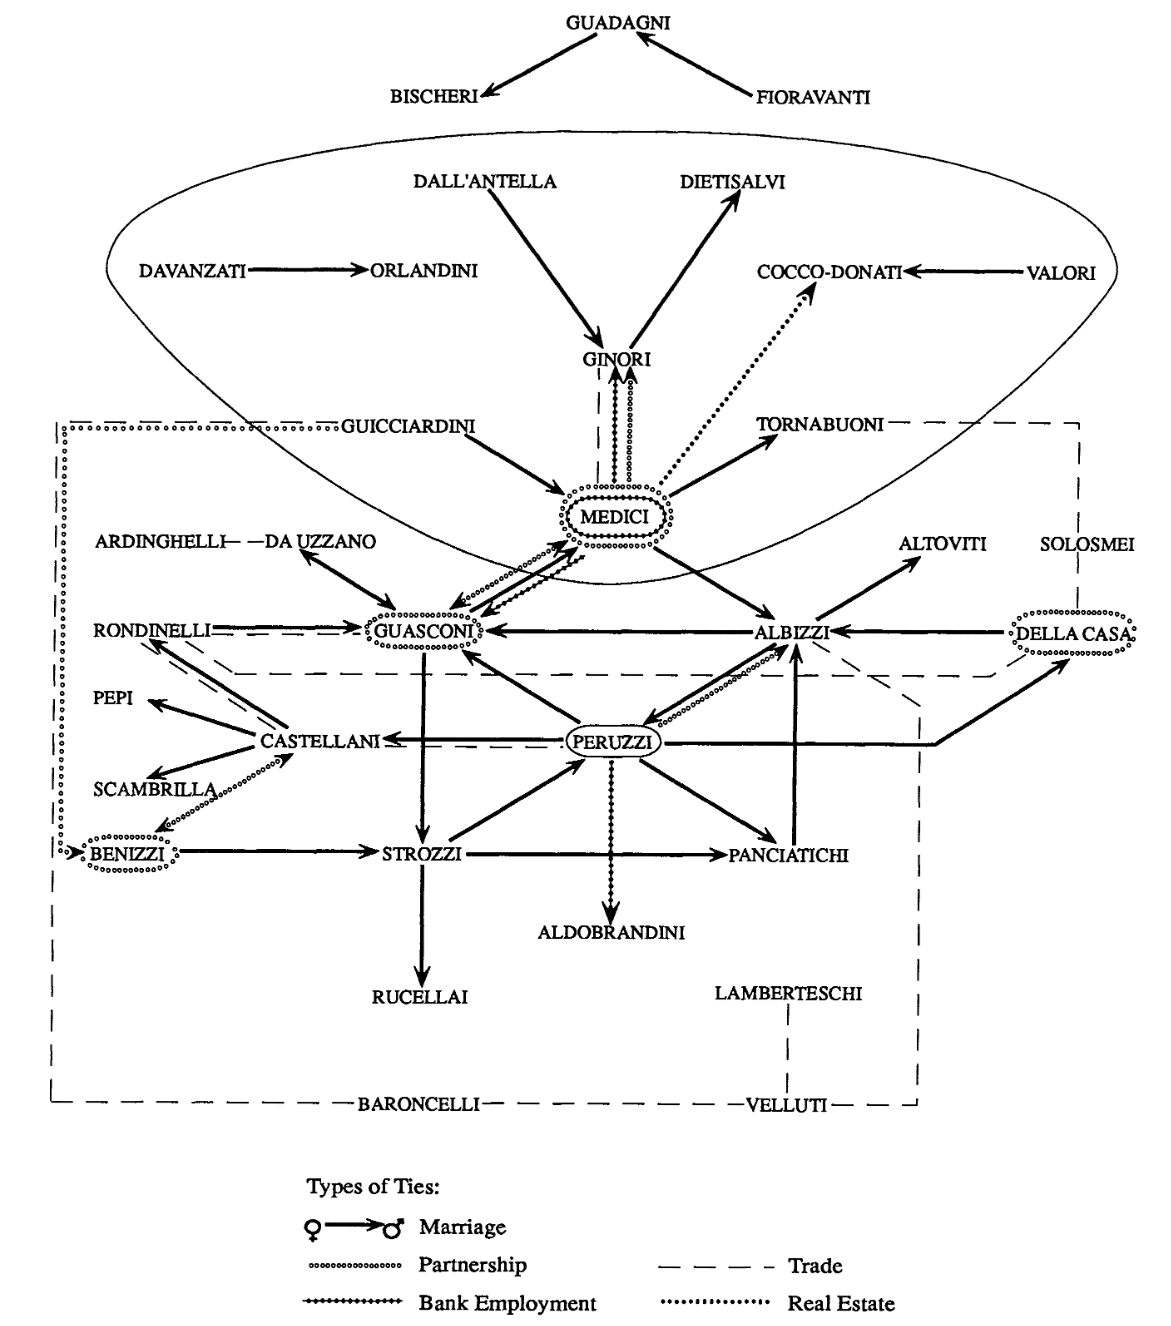
\includegraphics[width=0.8\textwidth]{static/figures/RelatedWork/padgett-Medicis.png}
%    \caption{Marriage, partnership. trading, banking, and real estate networks of the powerful families of Florence from \cite{padgettRobustActionRise1993}. We can see the central position in the network of the Medici Family.}
%    \label{fig:padgett-medicis}
%\end{figure}
\begin{figure}[!ht]
    \centering % avoid the use of \begin{center}...\end{center} and use \centering instead (more compact)
    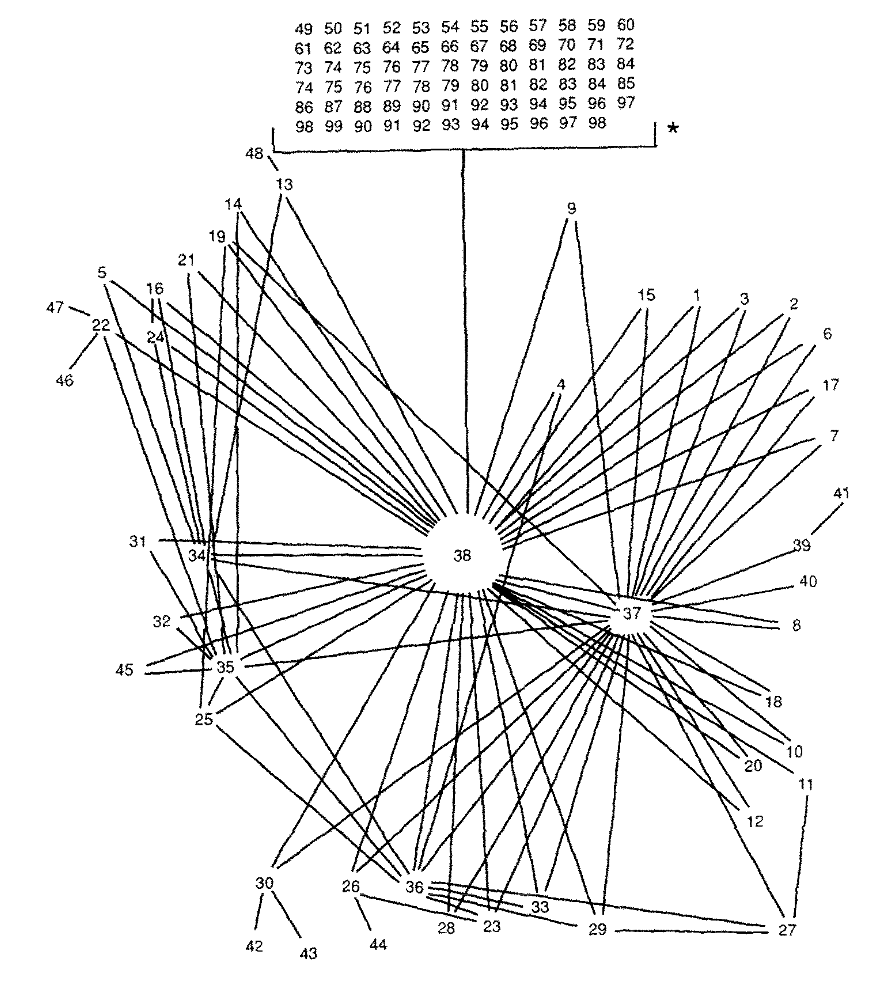
\includegraphics[width=0.8\textwidth]{static/figures/RelatedWork/Cicero_network}
    \caption{Cicero's personal communication network represented with a node-link diagram. Image from \cite{alexanderAnalysisAncientNetwork1990}}
    \label{fig:cicero-letters}
\end{figure}


Several historians are using and continuously reflecting on \hsna methods\cite{lemercier12FormalNetwork2015} which can be very effective to study relational historical phenomena~\cite{kerschbaumerPowerNetworksProspects2015}.
Moreover, historians rarely rely on a single approach when studying an era or phenomenon, they mix methods and tools from several domains of social and natural sciences with their own practices~\cite{padgettRobustActionRise1993, petzCombiningNetworkResearch2022}.




%However, constructing a network from historical sources, which can differ in their structure is not a trivial task.
%The most straightforward approach, based on the most well known social network analysis, consists in constructing social network based on simple graph $G = (V, E)$ with $V$ a set a vertices representing the persons of interest, and $E \subseteq V^2$ a set of edges modeling the social ties between pairs of persons.
%This allows to have a simple network to visualize and analyze, but does not always reflect the social complexity of the real relationships.
%More complex networks models have been proposed in SNA to be able to model more complex social relationships.


\subsection{Network Modeling}\label{subsec:network-modeling}

Constructing a network from historical documents, which can vary tremendously in their formats and structures, is not a trivial task\cite{alkadi2022}.

The most straightforward and well-known approach consists in constructing a network based on a simple graph such as in \autoref{eq:graph}, where the nodes are the persons extracted from the documents and a link is created when a mention of a social relationship is mentioned in the document (or if they appear in the same document)\cite{lemercier12FormalNetwork2015, bouletBatchKernelSOM2008}.
%The most straightforward and well-known approach consists in constructing a network based on a simple graph $G = (V, E)$ with $V$ a set of vertices representing the actors of interest (very often individuals mentioned in the documents), and $E \subseteq V^2$ a set of edges modeling the social ties between pairs of actors.
This enables to have a simple network to visualize and analyze, but it does not always reflect the sociological complexity of information contained in the documents.
%More complex networks models have been proposed in SNA and HNR to be able to model more complex social relationships.
\hsna network models have evolved over time to better take into account concrete properties of social networks, such as the importance of actors or relations with weighted networks, multiple relationships with multiplex networks, and dynamics of relations with dynamic networks.

Weighted networks model the importance of relations, with a weight $w$ attributed to each edge $e = (u, v, w)$, with $u, v \in V$, $e \in E$, and $w > 0$.
Multiplex networks allow the modeling of multiple kinds of relationships between actors, such as spouses and witnesses relations for a historical network constructed from marriage acts.
In that case, each edge $e = (u, v, d)$ of the graph
\begin{equation}
    G = (V, E, D)
\end{equation}
have a type $d \in D$ which characterize the relation. In the example of marriages, $D = \{spouse, witness\}$.
Most relations extracted from historical documents also often contain time information, which can be modeled into dynamic networks.
Many dynamic network models have been proposed\cite{rossettiCommunityDiscoveryDynamic2018}, depending if the time is encoded in the nodes, the links, or both, and if entities have a discrete or interval time.
As it is often hard to infer the end of social relationships from the trace of historical documents, we only consider in this thesis models which give a timestamp to either nodes or edges, such that
\begin{equation}
    G = (V, E, T)
\end{equation}
with vertices consisting of tuples $(u, t)$ and edges of triples $(u, v, t)$, with $t \in T$.

Bipartite networks have been proposed to model relations between two types of entities, such as organizations and employees where the relations link employees to organizations but not employees to employees or organizations to organizations\cite{borgattiSocialNetworkAnalysis2009}.
Formally, each node of the graph
\begin{equation}
    G = (V, E, B)
\end{equation}
have a type $b \in B$, with $card(B) = 2$. For each edge $e = (u, v) \in E$, the types $b_u$ and $b_v$ of $u$ and $v$ are not equal $b_u \neq b_v$.
Many social situations or documents can be modeled in these terms (%\textit{Interlocking directorates},
affiliation lists or co-authoring).
Multivariate networks, \ie graphs, where vertices and edges can be assigned multiple ``properties'' or ``attributes'', are less used in SNA\@.
These attributes are often considered secondary, the emphasis of SNA being on the topology, its features, measures, and evolution.

Historians, demographers, sociologists, and anthropologists have also been designing specific data models for their social networks, based on genealogy or more generally kinship~\cite{hambergerKinshipNetworkAnalysis2011}.
For genealogy, the standard GEDCOM~\cite{gedcom} format models a genealogical graph as a bipartite graph with two types of vertices: individuals and families.
This format also integrates an ``event'' object but it is diversely adapted in genealogical tools.
The Puck software~\cite{hambergerScanningPatternsRelationship2014} has extended its original genealogical graph with the concept of ``relational nodes'' to adapt the data model to more family structures and to integrate other social relationships for anthropology and historical studies.

When creating a network, sociologists and anthropologists can use direct observations of the real world, which is not the case for historians who only have access to biased and partial sources.
Indeed, the documents historians inspect are often produced by the political and economical elite of the time, and include the subjective view of the authors, especially for literary sources (letters, journals, books, etc.).
Historians, therefore, need to take a critical view of the sources by acknowledging the position of the authors of the documents compared to the rest of the society and include it in the analysis\cite{lemercierQuantitativeMethodsHumanities2019}.
Furthermore, the partiality of the sources often does not allow to have access to all possible relationship types of individuals.
For example, if many formal relations can be extracted from official documents such as marriage acts and censuses, informal relations such as friendships can exist without leaving any written trace\cite{lemercier12FormalNetwork2015}.
Even for official relationships such as parents and witnesses, there are high chances for missing documents, which do not allow to make too general and finite claims, such as ``X is always the case'' or ``XX is never the case''\cite{alexanderAnalysisAncientNetwork1990}.
Social historians, therefore, have to take into account the partiality and ambiguity of their sources in their analysis, in order to avoid including the bias inherent to their data in their high-level historical conclusions.




\section{Social Network Visualization}\label{sec:social-network-visualization}


Practitioners of \sna and \hsna have always visually depicted their network data for validation, exploration, and communication, mostly using node-link diagrams.
With the use of more complex network models and the increase in average network size and density, new visualization techniques have been proposed to represent the diversity of studied networks.
Moreover, more and more social scientists are following exploratory approaches using Visual Analytics (VA) tools, to describe more in-depth their data and generate new interesting hypotheses, using interaction and exploration capabilities.

\subsection{Graph Drawing}

Sociologists rapidly saw the potential of graphically showing relationships between individuals, to better comprehend the underlying social structure and communicate their findings\cite{freemanVisualizingSocialNetworks2000}.
Moreno elaborated sociograms to visually show friendships among schoolchildren with circles and lines to respectively show children and friendships ties \cite{morenoWhoShallSurvive1934}.
This type of representation---commonly called node-link diagram---is the most widely used in social sciences, as it is rapidly understandable and effective for small to medium-sized networks which are predominant in social sciences.
%The most used social network visualization softwares such as Gephi\cite{Gephi} and NodeXL\cite{noauthor_nodexl_nodate} are based on this type of representation and allow an integrated exploration and analysis with the help of various algorithms.
Finding an optimal placement for the nodes is however not that simple as several metrics can be optimized depending on the desired drawing, such as the number of edge crossings, the variance of edge length, orthogonality of edges, etc~\cite{cristofoliPrincipesUsagesDessins, kosakAutomatingLayoutNetwork1994}. \autoref{fig:kosak-graph-drawing} shows some of these metrics, synthesized by Kosara and al.~\cite{kosakAutomatingLayoutNetwork1994}.
\begin{figure}
    \centering % avoid the use of \begin{center}...\end{center} and use \centering instead (more compact)
    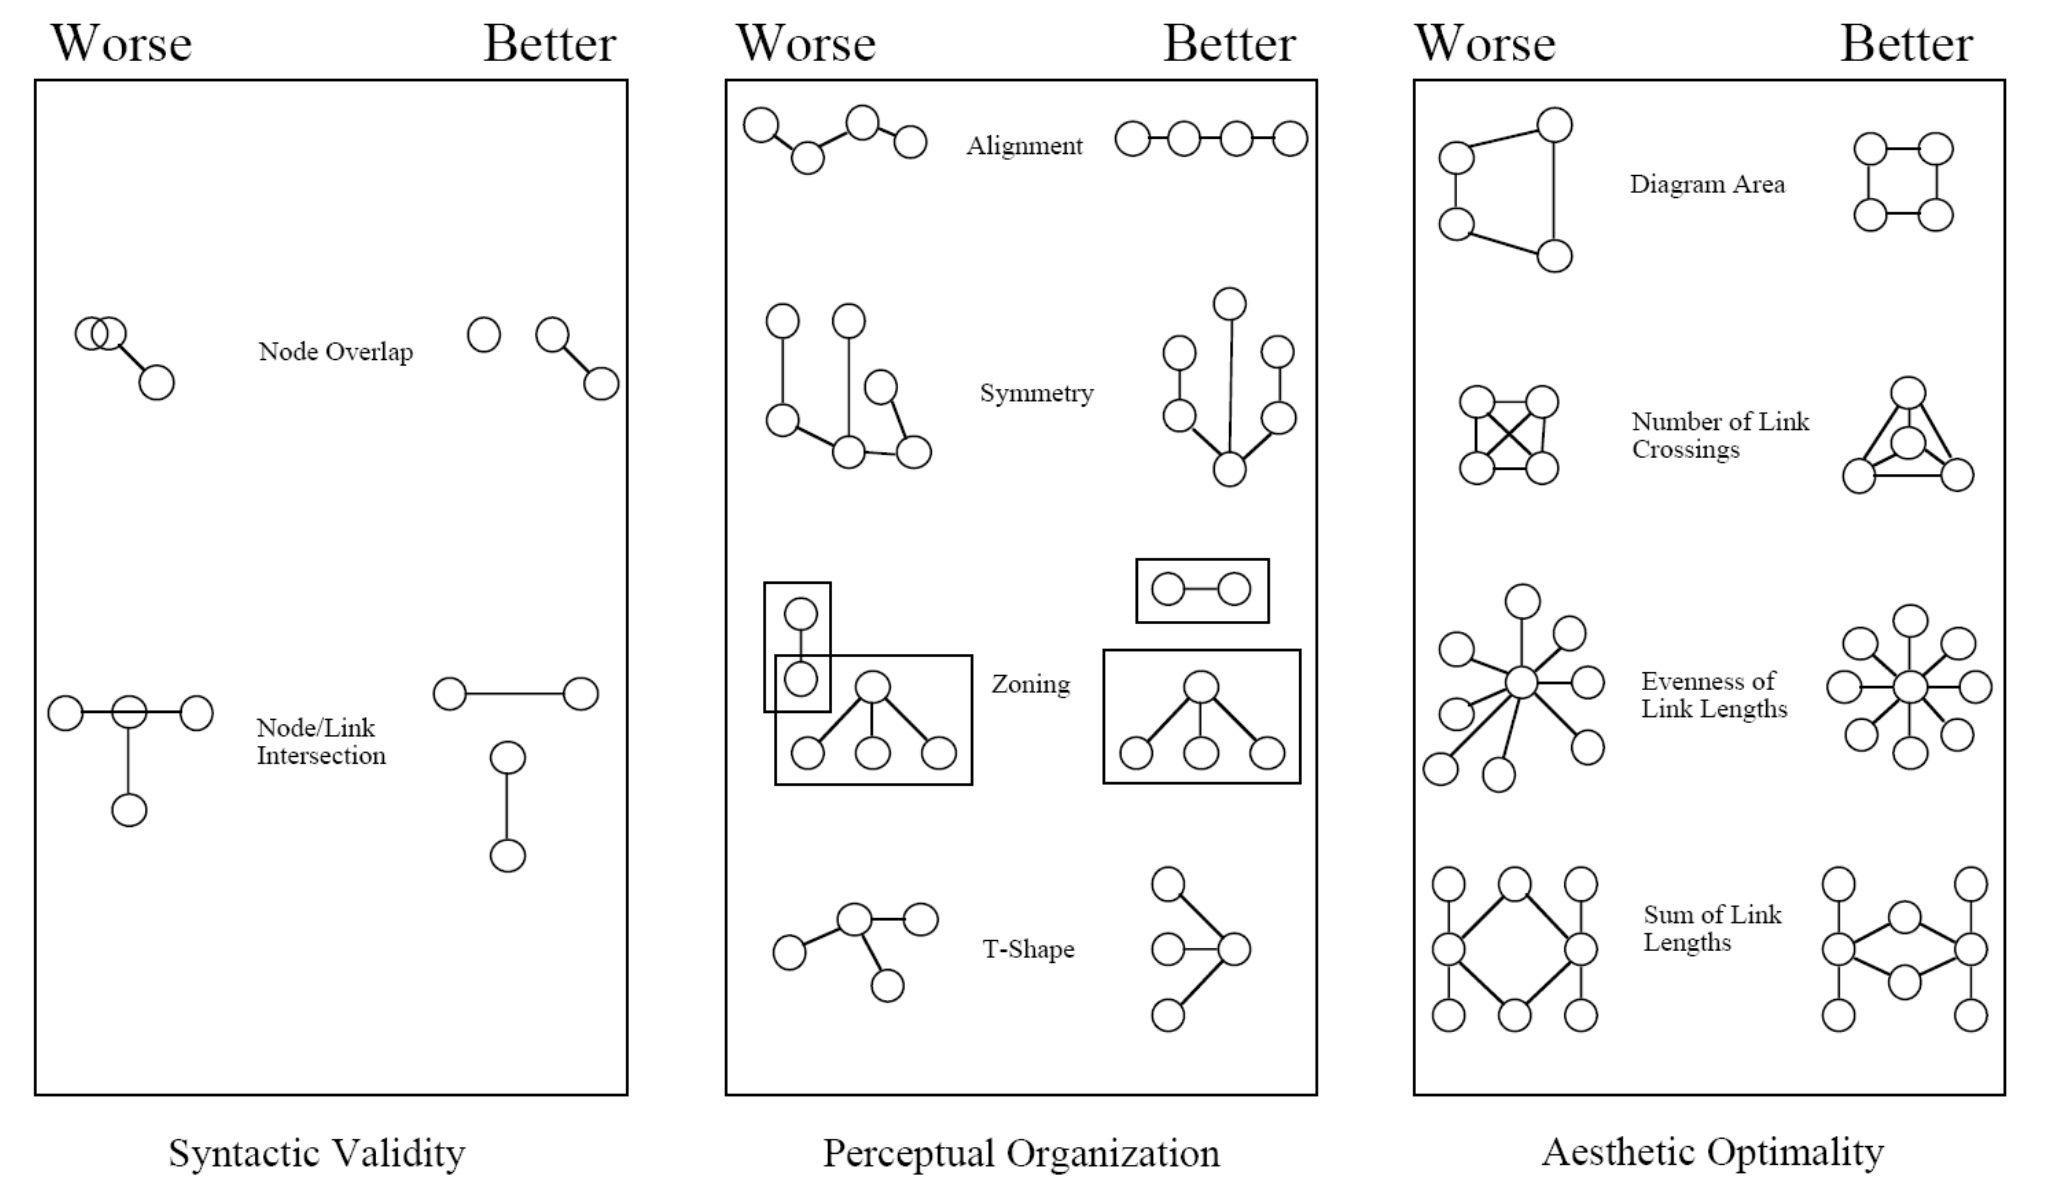
\includegraphics[width=1\textwidth]{static/figures/RelatedWork/Kosak-nodelinkdiagramMetrics}
    \caption{Different criteria are proposed to enhance node-link diagram readability. Image from \cite{kosakAutomatingLayoutNetwork1994}}
    \label{fig:kosak-graph-drawing}
\end{figure}
In \autoref{fig:moreno-sociogram} we can see the difference in readability between the original manual layout (left) and an automatic one (right).
Automatic layouts which aim at optimizing readability metrics give clearer diagrams.
The number of edge crossings is often considered the most important measure, but finding a drawing with the optimal number of crossings is an NP-Hard problem, meaning that heuristics are needed for most real-world use cases.
A large number of algorithms have been designed such as force-directed ones\cite{battistaGraphDrawingAlgorithms1998}, modeling the nodes as particles that repulse each other and are attracted together when connected with a link that can be seen as strings.
Other visual techniques have been proposed to represent networks such as matrices, circular layouts, and arcs, but are less used in social sciences \cite{mcguffinSimpleAlgorithmsNetwork2012}.
Still, Matrices have been shown to be more effective than node-link diagrams for several tasks such as finding cluster-related patterns, especially for medium to large networks \cite{ghoniemComparisonReadabilityGraphs2004, abdelaalComparativeEvaluationBipartite2022}.


As social scientists are using more complex network models such as bipartite or temporal networks, more sophisticated representations are needed.
%The visualization community proposed new visualization systems for specific network types such as PAOHVis for temporal hypergraphs, NodeTrix for clustered networks or Juniper for Multivariate networks.
The visualization community developed new representations to visualize other network types such as dynamic hypergraphs with PAOHVis \cite{valdiviaAnalyzingDynamicHypergraphs2021}, clustered graphs with NodeTrix \cite{henryNodeTrixHybridVisualization2007} (illustrated in \autoref{fig:Riche-NodeTrix}), geolocated social networks with the Vistorian \cite{serranomolineroUnderstandingUseVistorian2017}, and multivariate networks with Juniper \cite{nobreJuniperTreeTable2019}.
However, these new network representations take time to be adopted by social scientists who rarely use them.
\begin{figure}
    \centering % avoid the use of \begin{center}...\end{center} and use \centering instead (more compact)
    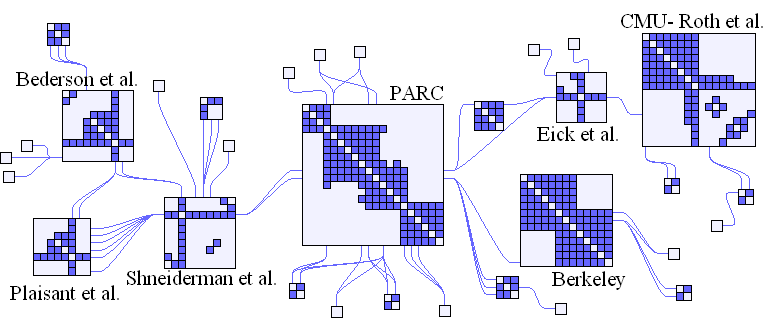
\includegraphics[width=0.8\textwidth]{static/figures/RelatedWork/NodeTrix.png}
    \caption{NodeTrix system showing a scientific collaboration social network with clusters. Each cluster is represented as a matrix,  Image from \cite{henryNodeTrixHybridVisualization2007}.}
    \label{fig:Riche-NodeTrix}
\end{figure}


\subsection{Social Network Visual Analytics}\label{subsec:social-network-visual-analytics}

Social scientists use visualization and analytical tools to gain insight on the structure of their finalized network data.
The most widely used tools are Gephi \cite{Gephi}, Pajek \cite{mrvarAnalysisVisualizationLarge2016}, Ucinet\cite{johnsonUCINETSoftwareTool1987}, and NodeXl \cite{NodeXL} which provide node-link diagrams, implementations of network measures, algorithms, and clustering capabilities.
Other \sna visualization tools have been proposed in the past such as Visone\cite{baurVisoneSoftwareVisual2002}.
However, those tools often do not include interaction and direct manipulation mechanisms, making the analysis more tedious for social historians and posing usability issues.
%Hence, they cannot be considered as purely \va interfaces as the analytical and visual components are not well integrated together.
In contrast, the Vistorian\cite{serranomolineroUnderstandingUseVistorian2017} let social historians visualize their network with multiple coordinated views (node-link, matrice, arc-diagram, and map), filters and direct manipulation, but do not integrate analytical options.
\autoref{fig:vistorian} shows the Vistorian interface used to explore a historical social network.
\begin{figure}[!ht]
    \centering % avoid the use of \begin{center}...\end{center} and use \centering instead (more compact)
    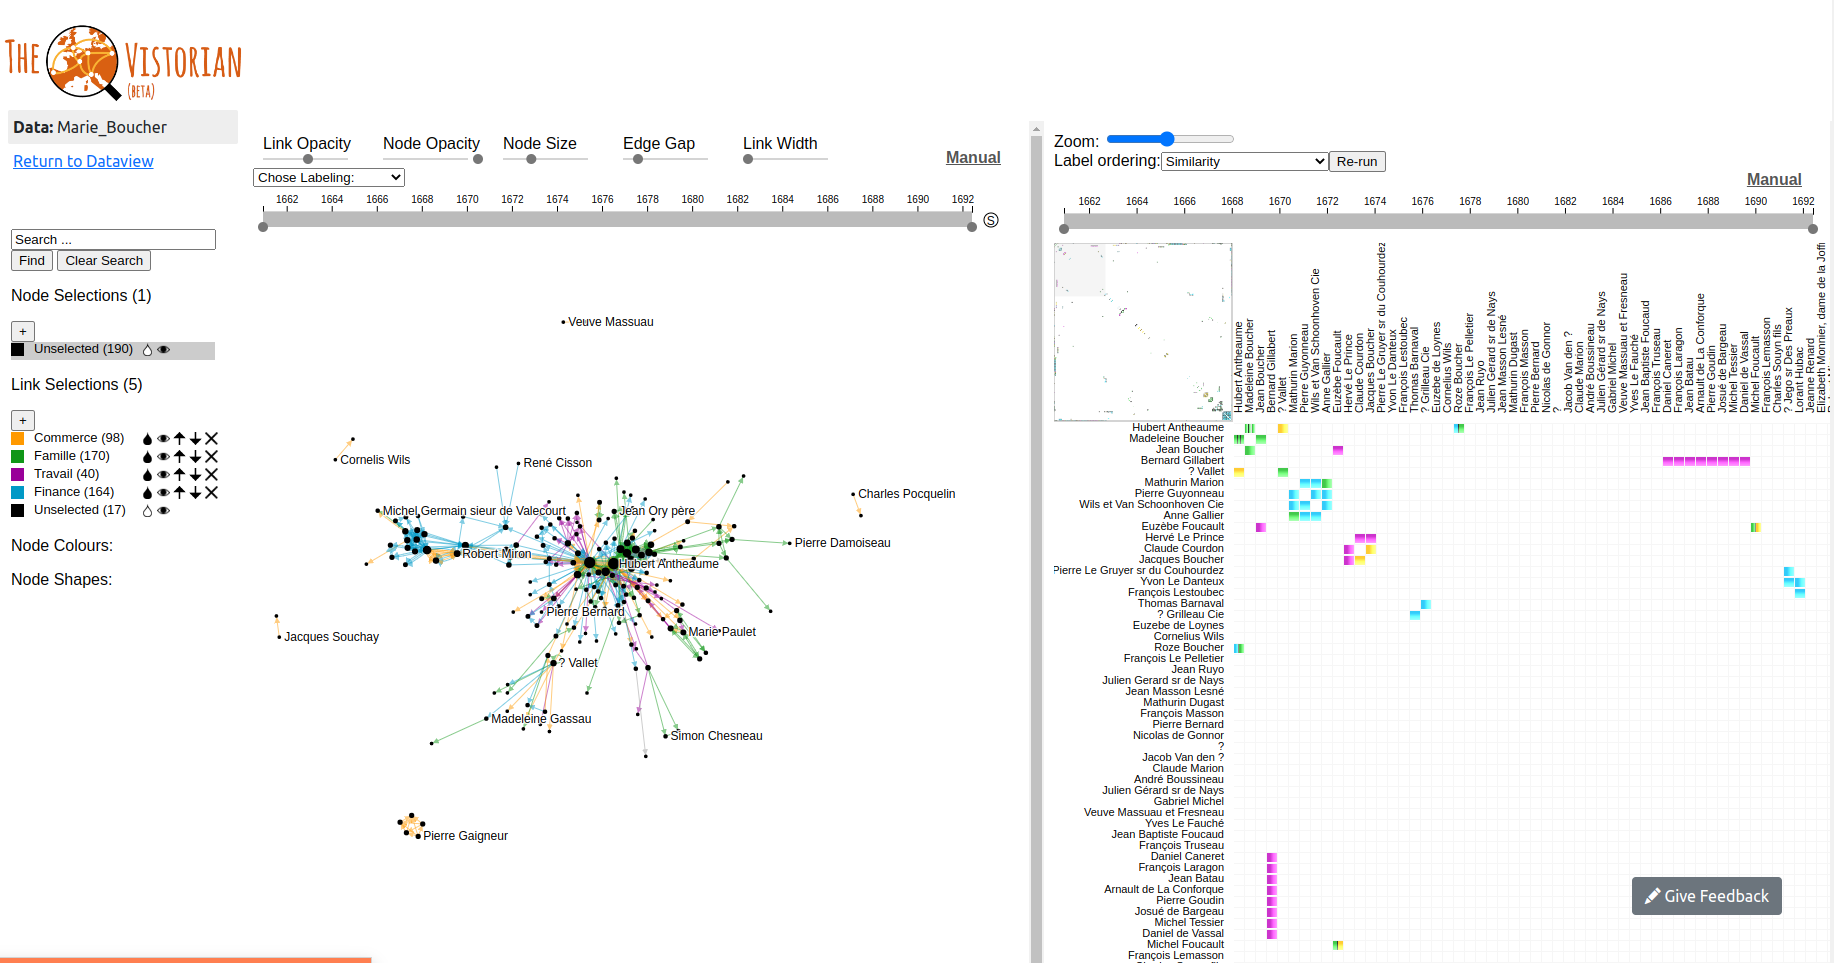
\includegraphics[width=1\textwidth,trim={0 1cm 0 0},clip]{static/figures/RelatedWork/vistorian}
    \caption{Vistorian interface\cite{serranomolineroUnderstandingUseVistorian2017} used to explore a historical social network of business trades in the 17th century, with a coordinated node-link diagram and a matrice view.}
    \label{fig:vistorian}
\end{figure}
%\includegraphics[trim={5cm 0 0 0},clip]{example-image-a}
I propose a classification of all those tools in \ref{tab:SNV}, which illustrate that the most used tools are analytical-oriented (Pajek, Ucinet, Gephi, NodeXl) while the Vistorian is an interactive visualization tool.
None of those softwares therefore fully correspond to the Visual Analytics label\cite{keimVisualAnalytics}.

\begin{table}[!ht]
\centering
\resizebox{\textwidth}{!}{%
\begin{tabular}{|l|l|l|l|l|l|}
\hline
 & Visualizations & \begin{tabular}[c]{@{}l@{}}SNA Measures \\ and Models\end{tabular} & Clustering & Filtering & Interaction/Direct Manipulation \\ \hline
Pajek     & \scaleone   & \scalethree & \scaletwo  & \scaleone   & \scalezero  \\ \hline
Ucinet    & \scaleone   & \scaletwo   & \scaleone  & \scalezero  & \scalezero  \\ \hline
Gephi     & \scaletwo   & \scaleone   & \scaleone  & \scaleone   & \scaleone   \\ \hline
NodeXl    & \scaleone   & \scaleone   & \scaletwo  & \scaleone   & \scalezero  \\ \hline
Vistorian & \scalethree & \scalezero  & \scalezero & \scalethree & \scalethree \\ \hline
\end{tabular}%
}
    \caption{Comparison table of most widely used visualization and analytical tool for \hsna. Visualizations: number of different visualization techniques, layouts, and interactions. \sna and Models: Number of proposed \sna measures and algorithms. Clustering: Number of proposed clustering algorithms. Filtering: Possibilities of filtering according to various criteria. Interaction/Direct Manipulation: Number of possible interaction mechanisms directly applicable to the visualizations. }
    \label{tab:SNV}
\end{table}
If analytical methods such as the computation of network measures, triad computation, or clustering provide a good framework to describe the structure of a network and link it to sociological explanation\cite{wassermanSocialNetworkAnalysis1994, scottSocialNetworkAnalysis1988}, many social scientists such as historians are not trained in computer science and mathematical methods and therefore have trouble to first use those methods without guidance, but also interpret their results.
This is particularly the case for black-box algorithms such as for clustering tasks: they usually end up trying several algorithms until they stumble upon a satisfactory enough solution\cite{pisterIntegratingPriorKnowledge2021}.

%Unfortunately, social scientists are often not trained in computer science and mathematical methods, and most of them have been frustrated by analytical and data mining tools and by how it was guiding their analysis in predefined ways.
%Particularly, the use of black-box algorithms such as for clustering tasks put analysts in an awkward position where they do not know how to interpret results.
%They usually end up trying several algorithms until they stumble upon a satisfactory enough solution\cite{pisterIntegratingPriorKnowledge2021}.

%Interfaces leveraging automatic data mining algorithms sometimes put users in an awkward position, as they have a hard time interpreting results coming from those black-box algorithms.
%They usually end up trying several algorithms until they stumble upon a satisfactory enough solution\cite{pisterIntegratingPriorKnowledge2021}.

Moreover, preparing and importing the data into visual and analytical software is complicated, as the annotation and network modeling process have not been globally formalized and every historian use different methods, formats and models.
Many users do not succeed in importing their data into those systems without concrete help and guidance\cite{serranomolineroUnderstandingUseVistorian2017, alkadi2022} due to mismatches with data models, formats, or data inconsistencies (null values, white spaces, etc.).
If they succeed in visualizing their data, it often shows them these inconsistencies or errors such as duplications of entities or wrong attribute values.
In other cases, they realize the network does not allow them to answer their sociological questions\cite{lemercier12FormalNetwork2015}.
%Thus, social scientists often encounter errors and inconsistencies in the data once they visualize it, that they want to correct.
It leads to continuous back and forth between their analysis process inside the analysis tool they are using, and their annotation/modeling process, to correct errors or modify annotations.
Interestingly, the network model choice plays a crucial role, as a simple network model representing only the persons (as is often the case) makes it harder to trace back to the original documents containing the annotations from the network entities.
Yet the majority of \sna systems enforce simple network models, making this retroactive process harder.

Some interfaces not primarily designed for social scientists incorporate data models encapsulating document representations, such as Jigsaw \cite{staskoJigsawSupportingInvestigative2008} which is a \va system using textual documents as a data model, originally developed for intelligence analysis.
It allows an analysis of the documents and their mentions of entities (persons, locations, institutions, etc.) through multiple coordinated views.
Using such a model allows us to rapidly see errors and inconsistencies in the document annotations that the user can directly correct, while still following complex analyzes.

Finally, more work is still to be done on social network \va tools, to provide more guidance and power to social scientists while doing their analysis, and to help them to do easier back and forth between the annotation, network modeling, correcting, and analysis steps, as errors and inconsistencies, can cause high variations in the network structure and hence the analysis results\cite{diesnerImpactEntityDisambiguation2015}.









%\autoref{fig:gephi} presents the Gephi interface showing a clustered social network, where each node is part of a cluster, encoded by color.
%
%\begin{figure}
%    \centering % avoid the use of \begin{center}...\end{center} and use \centering instead (more compact)
%    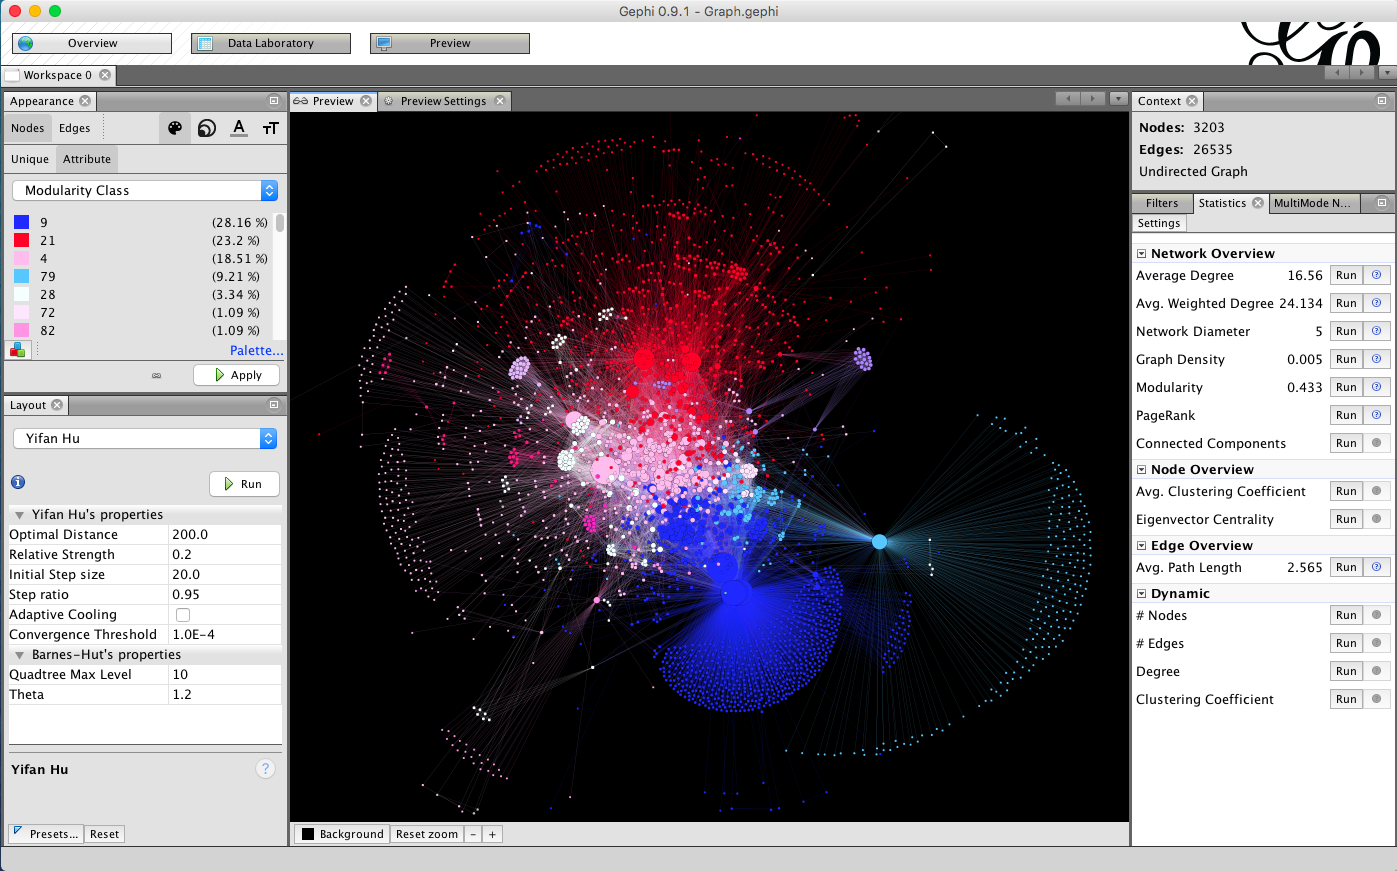
\includegraphics[width=0.8\textwidth]{static/figures/RelatedWork/Gephi_0.9.1_Network_Analysis_and_Visualization_Software}
%    \caption{Gephi \cite{Gephi} interface. The network is represented with a node-link diagram. Users can interact on the visualization and encode node and links visual attribute (color, size etc.) with network measures computed directly in the interface, such as the node degree, or clustering results.}
%    \label{fig:gephi}
%\end{figure}


%More complex \va interface have been proposed to explore social networks with complex interactions and more complex network models such as GUESS\cite{adarGUESSLanguageInterface2006} and the Vistorian\cite{serranomolineroUnderstandingUseVistorian2017}.
%These interfaces let social scientists explore their data with other interactions such as filtering, and often propose multiple coordinated views allowing to see the data through different lens.
%For example, the Vistorian can show the data using a node-link diagram, a matrix, a map, and arc diagrams.




%Most widely used social network visualization softwares by social scientists are Gephi \cite{Gephi}, Pajek \cite{mrvarAnalysisVisualizationLarge2016}, and NodeXl \cite{NodeXL} which provide node-link diagrams, and allow basic interactions such as selection to explore the network.
%These softwares usually provides automatic computation of several network measures such as the density and the diameter, allowing users to follow SNA workflows all in the interface.
%Similarly, Automatic clustering capabilities are provided letting users find interesting community structure in their network.
%
%More complex VA interface have been proposed to explore social networks with complex interactions and more complex network models such as GUESS\cite{adarGUESSLanguageInterface2006} and the Vistorian\cite{serranomolineroUnderstandingUseVistorian2017}.
%These interfaces let social scientists explore their data with other interactions such as filtering, and often propose multiple coordinated views allowing to see the data through different lens.
%For example, the Vistorian can show the data using a node-link diagram, a matrix, a map, and arc diagrams.
%These interfaces are usually aimed at more complex model than simple network,